% +-------------------------------\right) -------------------------------------+
% | LaTeX Template                                                     |
% | for K-State Electronic Theses, Dissertations, and Reports          |
% |                                                                    |
% | Comments and guidelines for using the template are shown           |
% | within boxes like this one.                                        |
% |                                                                    |
% | Revised 6/30/06                                                    |
% | 9/14/06: Removed typos                                             |
% +--------------------------------------------------------------------+

\documentclass[final, 12pt,oneside]{class_diss}

\usepackage[utf8]{inputenc}
\usepackage[T1]{fontenc}
\usepackage[spanish]{babel}
% +--------------------------------------------------------------------+
% | Now, we add in all external packages that we will use throughout   |
% | the document.  You can add other packages as needed.
% +--------------------------------------------------------------------+

%\usepackage{     caption2} % Customize captions a bit more
\usepackage{      amsmath} % American Mathematics Society standards
%\usepackage{      wrapfig} % Wraps text around a figure or table
\usepackage{     graphicx} % Extended graphics package.
%\usepackage{     fancyhdr} % Efficiently handles headers and footers
%\usepackage{       braket} % Bra-Ket notation package
%\usepackage{     mathrsfs} % Specialized Math fonts (Hamiltonian, etc.)
%\usepackage{boxedminipage} % Boxed text can be produced
%\usepackage{     setspace} % Controls line spacing via \begin{space}

\usepackage{amsxtra}
\usepackage{amssymb}
\usepackage{amsthm}
\usepackage{latexsym}
\usepackage{listings}

% +--------------------------------------------------------------------+
% | The color package allows one to select colors for hyperlinking     |
% | (see below).                                                       |
% +--------------------------------------------------------------------+

\usepackage[usenames]{color}

% +--------------------------------------------------------------------+
% | Colors defined for use with this template.                         |
% +--------------------------------------------------------------------+

\definecolor{  Pink}{rgb}{1.0, 0.5, 0.5}
\definecolor{Maroon}{rgb}{0.8, 0.0, 0.0}

\usepackage[pdftex, plainpages=false, pdfpagelabels]{hyperref}

\hypersetup{
    linktocpage=true,
    colorlinks=true,
    bookmarks=true,
    citecolor=blue,
    urlcolor=red,
    linkcolor=Maroon,
    citebordercolor={1 0 0},
    urlbordercolor={1 0 0},
    linkbordercolor={.7 .8 .8},
    breaklinks=true,
    pdfpagelabels=true,
}

% +--------------------------------------------------------------------+
% | Page margins are set on 1 inch on all sides.                       |
% +--------------------------------------------------------------------+

\topmargin      = -0.56in
\textheight     =  8.60in
\textwidth      =  6.46in
\oddsidemargin  =  0.02in

% +--------------------------------------------------------------------+
% | The document finally begins here.                                  |
% +--------------------------------------------------------------------+
\begin{document}

  \setcounter{page}{-1}

% +--------------------------------------------------------------------+
% | Title Page
% +--------------------------------------------------------------------+
% +--------------------------------------------------------------------+
% | Title Page
% +--------------------------------------------------------------------+

\newpage

% +--------------------------------------------------------------------+
% | This page should not contain a page number.  We use the
% | \thispagestyle[empty] command below to suppress page numbers
% | and other style elements.
% +--------------------------------------------------------------------+

\thispagestyle{empty}

% +--------------------------------------------------------------------+
% | The Title page begins here.
% +--------------------------------------------------------------------+

\begin{center}

   \vspace{1cm}

   {\Large Predicción a corto plazo de la energía
   	 generada por una placa solar}\\

   \vspace{0.5cm}

   \vspace{0.5cm}

   {\large Pablo Aragón Moreno}\\
   {\large María Castañeda López}\\
   {\large Abel Coronado López}\\
 
   \vspace{0.5cm}

   GRADO EN INGENIERÍA INFORMÁTICA. FACULTAD DE INFORMÁTICA\\
   UNIVERSIDAD COMPLUTENSE DE MADRID \\


   \vspace{0.65cm}
   \rule{2in}{0.5pt}\\
   \vspace{0.85cm}

  \includegraphics[height=2.5in]{figures/escudo.jpg}
  

   \vspace{0.5cm}
Trabajo Fin de Grado en Ingeniería Informática

   \vspace{0.5cm}

% +--------------------------------------------------------------------+
%  Fecha 
% +--------------------------------------------------------------------+

  16 de Junio de 2017\\
   \vspace{1cm}

\end{center}

{\raggedleft
Director/es y/o colaborador:\\
   \vspace{ 1cm}
José Ignacio Gómez\\
Christian Tenllado\\
}


% +--------------------------------------------------------------------+
% | Use the section below if you have co-major professors.
% +--------------------------------------------------------------------+

%\begin{flushleft}
%   \hspace{10cm}Approved by:\\
%   \vspace{ 1cm}
%   \hspace{10cm}Co-Major Professor\\
%   \hspace{10cm}Enter Your Co-Major Professor's Name\\
%   \vspace{.5cm}
%   \hspace{10cm}Co-Major Professor\\
%   \hspace{10cm}Enter Your Co-Major Professor's Name\\
%\end{flushleft}

   \pdfbookmark[0]{Portada}{PDFPortadaPage}

% +--------------------------------------------------------------------+
% | Authorizacion Page
% +--------------------------------------------------------------------+
% +--------------------------------------------------------------------+
% | Copyright Page
% +--------------------------------------------------------------------+

\newpage

\thispagestyle{empty}

\begin{center}

{\bf \Huge Autorización de difusión}

\vspace{1cm}

    {\large Pablo Aragón Moreno}\\
    {\large María Castañeda López}\\
    {\large Abel Coronado López}\\

   \vspace{0.5cm}

   16 de Junio de 2017\\
   \vspace{0.5cm}

\end{center}
   
El/la abajo firmante, matriculado/a en el Grado en Ingeniería Informática de la Facultad de Informática, autoriza a la Universidad Complutense de Madrid (UCM) a difundir y utilizar con fines académicos, no comerciales y mencionando expresamente a su autor el presente Trabajo Fin de Grado: “Predicción a corto plazo de la energía
    generada por una placa solar”, realizado durante el curso académico 2016-2017 bajo la dirección de Jose Ignacio Gómez, y a la Biblioteca de la UCM a depositarlo en el Archivo Institucional E-Prints Complutense con el objeto de incrementar la difusión, uso e impacto del trabajo en Internet y garantizar su preservación y acceso a largo plazo.

\vspace{2cm}

{\large Pablo Aragón Moreno}

\vspace{2.5cm}

{\large María Castañeda López}

\vspace{2.5cm}

{\large Abel Coronado López}

\vspace{2.5cm}

{\large Director: Jose Ignacio Gómez} \hspace{2cm} {\large Director: Christian Tenllado}
   \pdfbookmark[0]{Autorización}{PDFAutorizacionPage}

   \input{resumen.tex}
   
   \pdfbookmark[0]{Resumen}{PDFResumenPage}

    \input{abstract.tex}
       \pdfbookmark[0]{Abstract}{PDFAbstractPage}
    \vfill

\newpage
\pagenumbering{roman}

\setcounter{page}{1}

\phantomsection
\addcontentsline{toc}{chapter}{Índice}

\tableofcontents

% +--------------------------------------------------------------------+
% | Acknowledgements Page
% +--------------------------------------------------------------------+
\newpage
\begin{center}
{\bf \Huge Agradecimientos}
\end{center}
\vspace{1cm}
\setlength{\baselineskip}{0.8cm}

A nuestros directores del proyecto Jose Ignacio Gómez y Christian Tenllado por su implicación, atención y paciencia. Siempre dispuestos a orientarnos a lo largo de todo el proyecto y de enseñarnos aquello que no conocíamos.


\phantomsection
\addcontentsline{toc}{chapter}{Agradecimientos}

\newpage
\pagenumbering{arabic}
\setcounter{page}{1}

% +--------------------------------------------------------------------+
% | Chapters
% +--------------------------------------------------------------------+
\cleardoublepage

\chapter{Introducción}
\label{makereference1}

Este proyecto tiene como objetivo predecir, a través de herramientas informáticas, la irradiación solar en un punto teniendo en cuenta factores geográficos y meteorológicos.

La irradiación solar se puede usar como entrada de modelos físicos para la predicción de la energía. De esta manera podremos saber lo que podría generar una placa solar en un momento dado.

Ya existen modelos teóricos para saber cual va a ser la irradiación solar en un lugar, a partir la inclinación de los rayos solares en función de la longitud, la latitud, el día del año, la hora del día y suponiendo un cielo en ausencia de nubes. Estos modelos no tienen en cuenta los factores climáticos que tienen un gran peso en la disipación de la radiación.

En la figura \ref{modelo_verano} podemos observar una gráfica en la que aparecen los resultados de distintos modelos teóricos de predicción de la radiación en el verano de 2015. La gráfica representa la radiación media de todo el verano durante las horas del día.

\begin{figure}[htb]
	\begin{center}
		\includegraphics[width=12cm]{figures/verano2015.png}
		\caption{Modelo verano 2015. \label{modelo_verano}} 
	\end{center}
\end{figure}

Aunque se observa en la gráfica que la predicción se acerca a la realidas, la radiación solar no solo se ve afectada por los parámetros de estos modelos. También varía debido a diversos factores de las variaciones locales en la atmósfera como por ejemplo el vapor de agua, las nubes o la contaminación. Este proyecto quiere acercar todavía más esta predicción haciendo uso de algunos de estos factores.

Para llevar a cabo esta predicción en este proyecto se han utilizado como variables atmosféricas la humedad, la temperatura y la propia radiación solar. La manera de resolver este problema han sido algoritmos de ``Machine Learning'' (explicados en el capítulo \ref{makereference5}).

\section{Motivación}
\label{makereference1.1}

Hoy en día es cada vez más importante el uso de las energías renovables y así, utilizar cada vez menos los combustibles fósiles. Esto es debido a que estas no producen gases de efecto invernadero que son los causantes del cambio climático, tampoco producen emisiones contaminantes, son inagotables y generan residuos fáciles de tratar.

También tienen algunos inconvenientes como, por ejemplo, el gran impacto visual que tienen y las grandes cantidades de terreno que se necesitan para poder conseguir una cantidad significante de energía. Además no siempre se obtiene la misma cantidad de energía. Depende, por ejemplo, de la cantidad de sol o de viento en ese momento.

Este último inconveniente es el que hace que las compañías productoras y distribuidoras sean reacias al uso de estas energías.

Debido a la liberalización del sector energético, la compra-venta de la energía se realiza en subastas cada hora. Las compañías, deben conocer su capacidad de producción para poder adecuarla a la demanda de estas subastas. Debido a la incertidumbre de cuánta energía se va a producir, es difícil desarrollar estrategias de compra de energía a otros productores y adecuación de su producción y capacidad de reserva.

En energías renovables como la eólica, los modelos predictivos disponibles actualmente son bastante precisos y su impulso es más fácil que otras como la energía solar la cual es más dificil de predecir.

Se podría decir que todavía no existen modelos realmente buenos para predecir la energía solar. Hay algunas empresas como \href{https://aleasoft.com/es/}{Aleasoft}, que realizan estudios predictivos obteniendo previsiones horarias en tiempo real desde un día hasta diez días, pero sería necesario conocer la producción con un intervalo de una o dos horas.

Para ello, este proyecto intenta predecir a corto plazo la radiación solar y poder aplicar esta en una instalación de granja solar.

\section{Breve descripción del sistema}
\label{makereference1.2}

Este sistema cuenta con cuatro grandes módulos de trabajo para llevar a cabo su función: nodo, servidor de datos, servidor de resultados y visualizador de datos. Ver figura \ref{diagrama-sistema}.

\subsection{Nodo}
\label{makereference1.2.1}
Encargado de recoger los datos necesarios, está formado por distintos sensores que recogen la información meteorológica necesaria y una pequeña placa programable encargada de enviar esta información al servidor de datos.

\subsection{Servidor de datos}
\label{makereference1.2.2}
El servidor de datos, es el encargado de recibir, almacenar y distribuir la información obtenida por el nodo.

\subsection{Servidor de predicción}
\label{makereference1.2.3}
Tiene como función recoger la información almacenada del servidor de datos, procesarla para obtener la predicción y enviarla al visualizador de datos. Puede estar, o no, en la misma máquina que el servidor de datos.

\subsection{Sistema de visualización}
\label{makereference1.2.4}
Muestra los resultados en forma de gráficas para facilitar su análisis.

\begin{figure}[htb]
    \begin{center}
        \includegraphics[width=15cm]{figures/diagrama-sistema.png}
        \caption{Diagrama de los componentes del sistema con sus protocolos de comunicación. \label{diagrama-sistema}}
    \end{center}
\end{figure}

\cleardoublepage

\chapter{Introduction}
\label{makereference2}

This project aims to predict, through computer tools, the solar radiation at one point taking into account geographic and meteorological factors.

There are already theoretical models to know how much solar irradiation will be in a place, from the inclination of the sun rays in the function of the length, the latitude, the day of the year, the time of day and assuming a sky in the absence of clouds. These models do not take into account the climatic factors that have a great weight in the dissipation of the radiation.

In the picture \ref{modelo_verano} we can observe a graph showing the results of different theoretical models of radiation prediction in the summer of 2015. The graph represents the average radiation of the whole summer during the hours of the day.

Although it is observed in the graph that the prediction approaches the reality, the solar radiation is not only affected by the parameters of these models. It also varies due to various factors of local variations in the atmosphere such as water vapor, clouds or pollution. This project wants to bring this prediction even closer by making use of some of these factors.

To carry out this prediction in this project, the humidity, temperature and the solar radiation itself have been used as atmospheric variables. The way to solve this problem have been algorithms of `` Machine Learning '' (explained in chapter \ref{makereference5}).

\section{Motivation}
\label{makereference2.1}

Nowadays, the use of renewable energies is becoming more and more important and, therefore, to use less and less fossil fuels. This is because they do not produce greenhouse gases that are the cause of climate change, they do not produce pollutant emissions, they are inexhaustible and generate waste easy to treat.

They also have some drawbacks, such as the great visual impact they have and the large amounts of land needed to get a significant amount of energy. In addition you do not always get the same amount of energy. It depends, for example, on the amount of sun or wind at that time.

This last drawback is that makes the producing and distributing companies are reluctant to use these energies.

Due to the liberalization of the energy sector, energy buying and selling takes place at hourly auctions. The companies must know their production capacity in order to adapt it to the demand of these auctions. Due to the uncertainty of how much energy is going to be produced, it is difficult to develop strategies to purchase energy from other producers and to adjust their production and reserve capacity.

In renewable energies such as wind, currently available predictive models are quite accurate and their momentum is easier than others such as solar energy which is more difficult to predict.

It could be said that there are still no really good models to predict solar energy. There are some companies like \href{https://aleasoft.com/es/}{Aleasoft}, that perform predictive studies obtaining real-time forecasts from one day to ten days, but it would be necessary to know the production with an interval of one or two hours.

For this reason, this project tries to predict in the short term the solar radiation and to be able to apply this in a solar farm installation.

\section{Brief description of the system}
\label{makereference2.2}
This system has four large work modules to perform its function: node, data server, results server and data viewer. View picture \ref{diagrama-sistema}.

\subsection{Node}
\label{makereference2.2.1}
In charge of collecting the necessary data, it is formed by different sensors that collect the necessary meteorological information and a small programmable board in charge of sending this information to the data server.

\subsection{Data server}
\label{makereference2.2.2}
The data server is responsible for receiving, storing and distributing the information obtained by the node.

\subsection{Prediction server}
\label{makereference2.2.3}
It has as function to collect the stored information of the data server, to process it to obtain the prediction and to send it to the data visualizer. It may or may not be on the same machine as the data server.

\subsection{Display system}
\label{makereference2.2.4}
Display the results in the form of graphs for easy analysis.
\cleardoublepage

\chapter{Servidor de datos}
\label{makereference3}

\section{Introducción}
\label{makereference3.1}
La información recogida por el nodo es almacenada en un servidor central (``servidor de datos''). Este se encarga de recibir la información proporcionada por uno o varios clientes (el nodo en nuestro caso), almacenarla y distribuirla a quién la requiera.

La comunicación se realiza sobre el protocolo MQTT, muy utilizado para la comunicación máquina a máquina. Como implementación de este protocolo utilizamos el servidor \href{https://mosquitto.org/}{mosquitto}.

Existen varias alternativas a esta tecnología como por ejemplo:
\begin{itemize}
\item \href{https://en.wikipedia.org/wiki/Constrained_Application_Protocol}{CoAP} (Constrained Application Protocol) es un protocolo que está diseñado para la transferencia de documentos entre dispositivos restringidos. Dentro de sus ventajas podemos destacar que está destinado para su uso en dispositivos de Internet con recursos limitados, está diseñado para traducir fácilmente a HTTP.
\item \href{https://www.amqp.org/}{AMQP} (Advanced Message Queuing Protocol) destaca por su orientación a la mensajería de negocios. Regula el comportamiento tanto del servidor como del cliente de la mensajería logrando que las implementaciones de diferentes proveedores sean interoperables. Esta es una de sus características más señaladas.
\end{itemize}

Al final nos decantamos por MQTT debido a sus ventajas frente a las alternativas expuestas:

\begin{itemize}
\item Sistema de suscripción. Esto permite poder tener muchos nodos sin un gran esfuerzo.
\item Utiliza un ancho de banda mínimo. Tiene una cabecera fija de 2 bytes más una cabecera variable. De este variable, durante la suscripción y conexión se utilizan 12 bytes. La mayoría de publicaciones utilizan 2 bytes de cabeceras variables.
\item Consume muy poca energía.
\item Permite una gran fiabilidad si es necesario por la definición de la QoS (Calidad de Servicio).
\item Es muy escalable.
\end{itemize}

Hemos implementado MQTT sobre la tecnología inalámbrica Wi-Fi. Debido a que el proyecto es un prototipo, no nos hemos preocupado por la optimización de recursos. De ser así, habríamos elegido otro tipo de tecnologías usadas en comunicaciones ``machine-to-machine'', como por ejemplo \href{https://www.lora-alliance.org/What-Is-LoRa/Technology}{LoRa}.

 LoRa (Long Range) es una tecnología que ofrece un largo alcance, un bajo consumo de energía y una transmisión segura de datos. Entre sus ventajas cabe señalar que permite aplicaciones de seguimiento sin GPS, tiene un bajo coste y una alta capacidad, ideal para operadores de redes públicas.

\section{MQTT}
\label{makereference3.2}
MQTT o lo que es lo mismo \textit{Message Queue Telemetry Transport}, es un protocolo para la comunicación ``machine-to-machine'' de mensajería muy simple y ligero, orientado a conexión por TCP/IP. Está diseñado principalmente para dispositivos con poco ancho de banda y con latencia baja.

MQTT es un servicio de publicación/suscripción TCP/IP sencillo y muy ligero. Se basa en el principio cliente/servidor y suscriptor/publicador.

El servidor, llamado broker, recopila los datos que los publicadores (``publishers'' en adelante) le transmiten. Determinados datos recopilados por el broker se enviarán a determinados publishers que previamente así se lo hayan solicitado al broker.

Los publishers envían los mensajes a un canal llamado topic. Los suscriptores (``subscribers'') pueden leer esos mensajes. Los topics (o canales de información) pueden estar distribuidos jerárquicamente de forma que se puedan seleccionar exactamente las informaciones que se desean.

La disposición jerárquica de estos ``topics'' está especialmente diseñada para facilitar la distribución de publishers y subscribers por grupos. De esta forma, si tuvieramos una instalación domótica, podríamos distribuir los elementos a controlar en grupos jerárquicos.

Los mensajes enviados por los dispositivos comunicantes pueden ser de todo tipo pero no pueden superar los 256 Mb.

\subsection{Seguridad}
Los datos de IoT intercambiados pueden resultar muy críticos, por lo que es posible garantizar la seguridad de los intercambios en varios niveles:

\begin{itemize}
\item Transporte en SSL/TLS.
\item Autenticación mediante certificados SSL/TLS.
\item Autenticación mediante usuario y contraseña.
\end{itemize}

\subsection{QoS}
El protocolo MQTT define tres modos diferentes de asegurar la Calidad del Servicio (QoS, Quality of Service) que el publicador podrá definir según sus necesidades.

Hay tres niveles posibles:
\begin{itemize}
\item QoS nivel 0 (At Most Once) se entregará como mucho una vez, por lo que el mensaje no tiene garantías de recepción (el broker no informa al publicador de que ha recibido el mensaje).

\item Qos nivel 1 (At Least Once) se entregará al menos una vez. El publicador lo transmitirá varias veces si es necesario, hasta que el broker le confirme que lo ha enviado a la red. Este es el nivel por defecto.

\item QoS nivel 2 (Exactly Once) será obligatoriamente guardado por el emisor, que lo transmitirá siempre que el receptor no confirme su envío a la red.

En este proyecto se usa QoS nivel 1, que es el que tiene ``mosquitto'' por defecto.

\end{itemize}
\begin{figure}[htb]
	\begin{center}
		\includegraphics[height=8cm]{figures/mqtt-qos.jpg}
		\caption{Diagrama de los distintos niveles de calidad [Fuente: \href{https://image.slidesharecdn.com/0xwitjksqnqruoz4tnsi-signature-6a256d24caf5d1fcc6a3bf1d013dfe0e1fa99369a560d140998f50cbdbc6d127-poli-140828123252-phpapp02/95/mqtt-a-practical-protocol-for-the-internet-of-things-15-638.jpg?cb=1409229409}{SlideShare: MQTT - A practical protocol for the Internet of Thing}] \label{qos}}
	\end{center}
\end{figure}

\cleardoublepage

\chapter{Servidor de datos}
\label{makereference4}

\section{Introducción}
\label{makereference4.1}
La información recogida por el nodo es almacenada en un servidor central (``servidor de datos''). Este se encarga de recibir la información proporcionada por uno o varios clientes (el nodo en nuestro caso), almacenarla y distribuirla a quién la requiera.

La comunicación se realiza sobre el protocolo MQTT, muy utilizado para la comunicación máquina a máquina. Como implementación de este protocolo utilizamos el servidor \href{https://mosquitto.org/}{mosquitto}.

Existen varias alternativas a esta tecnología como por ejemplo:
\begin{itemize}
\item \href{https://en.wikipedia.org/wiki/Constrained_Application_Protocol}{CoAP} (Constrained Application Protocol) es un protocolo que está diseñado para la transferencia de documentos entre dispositivos restringidos. Dentro de sus ventajas podemos destacar que está destinado para su uso en dispositivos de Internet con recursos limitados, está diseñado para traducir fácilmente a HTTP.
\item \href{https://www.amqp.org/}{AMQP} (Advanced Message Queuing Protocol) destaca por su orientación a la mensajería de negocios. Regula el comportamiento tanto del servidor como del cliente de la mensajería logrando que las implementaciones de diferentes proveedores sean interoperables. Esta es una de sus características más señaladas.
\end{itemize}

Al final nos decantamos por MQTT debido a sus ventajas frente a las alternativas expuestas:

\begin{itemize}
\item Sistema de suscripción. Esto permite poder tener muchos nodos sin un gran esfuerzo.
\item Utiliza un ancho de banda mínimo. Tiene una cabecera fija de 2 bytes más una cabecera variable. De este variable, durante la suscripción y conexión se utilizan 12 bytes. La mayoría de publicaciones utilizan 2 bytes de cabeceras variables.
\item Consume muy poca energía.
\item Permite una gran fiabilidad si esta es necesaria, por la definición de la QoS (Calidad de Servicio).
\item Es muy escalable.
\end{itemize}

\section{MQTT}
\label{makereference4.2}
MQTT o lo que es lo mismo \textit{Message Queue Telemetry Transport}, es un protocolo para la comunicación ``machine-to-machine'' de mensajería muy simple y ligero, orientado a conexión por TCP/IP. Está diseñado principalmente para dispositivos con poco ancho de banda y con latencia baja.

MQTT es un servicio de publicación/suscripción TCP/IP sencillo y muy ligero. Se basa en el principio cliente/servidor y suscriptor/publicador.

El servidor, llamado broker, recopila los datos que los publicadores (``publishers'' en adelante) le transmiten. Determinados datos recopilados por el broker se enviarán a determinados publishers que previamente así se lo hayan solicitado al broker.

Los publishers envían los mensajes a un canal llamado topic. Los suscriptores (``subscribers'') pueden leer esos mensajes. Los topics (o canales de información) pueden estar distribuidos jerárquicamente de forma que se puedan seleccionar exactamente las informaciones que se desean.

La disposición jerárquica de estos ``topics'' está especialmente diseñada para facilitar la distribución de publishers y subscribers por grupos. De esta forma, si tuvieramos una instalación domótica, podríamos distribuir los elementos a controlar en grupos jerárquicos.

Los mensajes enviados por los dispositivos comunicantes pueden ser de todo tipo pero no pueden superar los 256 Mb.

\subsection{Seguridad}
Los datos de IoT intercambiados pueden resultar muy críticos, por lo que es posible garantizar la seguridad de los intercambios en varios niveles:

\begin{itemize}
\item Transporte en SSL/TLS.
\item Autenticación mediante certificados SSL/TLS.
\item Autenticación mediante usuario y contraseña.
\end{itemize}

\subsection{QoS}
El protocolo MQTT define tres modos diferentes de asegurar la Calidad del Servicio (QoS, Quality of Service) que el publicador podrá definir según sus necesidades.

Hay tres niveles posibles:
\begin{itemize}
\item QoS nivel 0 (At Most Once) se entregará como mucho una vez, por lo que el mensaje no tiene garantías de recepción (el broker no informa al publicador de que ha recibido el mensaje).

\item Qos nivel 1 (At Least Once) se entregará al menos una vez. El publicador lo transmitirá varias veces si es necesario, hasta que el broker le confirme que lo ha enviado a la red. Este es el nivel por defecto.

\item QoS nivel 2 (Exactly Once) será obligatoriamente guardado por el emisor, que lo transmitirá siempre que el receptor no confirme su envío a la red.

En este proyecto se usa QoS nivel 1, que es el que tiene ``mosquitto'' por defecto.

\end{itemize}
\begin{figure}[htb]
	\begin{center}
		\includegraphics[height=8cm]{figures/mqtt-qos.jpg}
		\caption{Diagrama de los distintos niveles de calidad [Fuente: \href{https://image.slidesharecdn.com/0xwitjksqnqruoz4tnsi-signature-6a256d24caf5d1fcc6a3bf1d013dfe0e1fa99369a560d140998f50cbdbc6d127-poli-140828123252-phpapp02/95/mqtt-a-practical-protocol-for-the-internet-of-things-15-638.jpg?cb=1409229409}{SlideShare: MQTT - A practical protocol for the Internet of Thing}] \label{qos}}
	\end{center}
\end{figure}

\cleardoublepage

\chapter{Exploración del modelo predictivo}
\label{makereference5}

\section{Introducción a los modelos predictivos}
\label{makereference5.1}

Cuando hablamos de modelos predictivos nos estamos refiriendo al análisis que agrupa una serie de técnicas para conseguir analizar datos reales tanto actuales como históricos y, así, conseguir predicciones. Con esta predicción podremos saber cuánto se acerca nuestro modelo a la realidad.

Existen algunos conceptos clave a la hora de hablar de metodos predictivos:
\begin{itemize}
	\item Conjunto de entrenamiento: son los datos a partir de los cuales se desarrollan los modelos predictivos.
	\item Conjunto de validación: datos utilizados para evaluar el rendimiento de dichos modelos.
	\item Predictores: variables de entrada, utilizadas para la ecuación de predicción. 
	\item Resultado: objetivo que se quiere predecir.
\end{itemize}

Las fases para desarrollar este tipo de modelos son las siguientes:
\begin{itemize}
\item Entrenamiento: para predecir con estas técnicas primero se debe ``entrenar'' el sitema. Esto se puede realizar de dos formas, proporcionando al entrenamiento los resultados ya conocidos de las predicciones (aprendizaje supervisado) o no (aprendizaje no supervisado). Más adelante se explicará en qué consiste este entrenamiento.

En este proyecto se utilizan algoritmos de aprendizaje supervisado.

Para realizar un ``entrenamiento supervisado'' se selecciona un conjunto de datos (conjunto de entrenamiento) del que se conoce el valor real de la predicción que queremos realizar y se explora, en función del algoritmo seleccionado, variando los parámetros internos del algoritmo para obtener un posible modelo.

Cada modelo tiene una serie de variables que podemos definir previas al entrenamiento que influirán en el resultado. En esta fase, los factores que se buscan explorar son aquellos que, internamente, ajusta el propio algoritmo en función de los datos de entrada y los parámetros que definamos.

\item Validación: se selecciona otro conjunto de datos distinto al anterior (conjunto de validación) del que también se conoce el valor real de la predicción y se aplica el modelo obtenido en el entrenamiento. Se comparan los datos proporcionados con el modelo con los datos reales y se sacan distintas métricas para conocer su efectividad. 

En función del resultado obtenido en la validación, se pueden volver a repetir estos dos pasos cambiando el conjunto de datos o los parámetros de entrada del modelo hasta conseguir una predicción óptima.

\item Predicción: una vez encontrado un modelo en la fase anterior que cumpla con los requisitos, se guarda ese modelo en algún formato recuperable para poder utilizarlo en cualquier momento sin tener que volver a entrenarlo.
\end{itemize}

Los algoritmos predictivos que se han estudiado han sido los siguientes:

\begin{itemize}
\item Regresión Lineal
\item SVR (Support Vector Regression)
\item Redes Neuronales
\end{itemize}

\section{Conjunto de datos}
\label{makereference5.2}

Para poder encontrar el modelo más adecuado para este problema se necesita una gran cantidad de datos con la que entrenar y validar. Estos datos han sido obtenidos de \href{http://www.inforiego.org/opencms/opencms}{InfoRiego}, una herramienta pensada para estudiar el consumo de agua en los cultivos y hacerlo más eficiente que proporciona la información meteorológica que necesaria para este proyecto.

``InfoRiego'' hace uso de la red de estaciones meteorológicas SIAR (proyecto de la Dirección General de Desarrollo Rural del Ministerio de Medio Ambiente y Medio Rural y Marino) y de las estaciones del ITACyL (Instituto Tecnológico Agrario de Castilla y León).

Hay dos formas de obtener los datos de InfoRiego: a través de una API Rest o a través de FTP.

Este proyecto realiza la consulta de datos a través del servidor FTP de inforiego. Este servidor proporciona acceso mediante HTTP por lo que se obtienen los archivos con la información meteorológica deseada a través de WebScrapping.

WebScrapping es una técnica que recorre, a través de software, los elementos HTML de un sitio web pudiendo así obtener su información.

Se ha creado un script en Python que, dados unos parámetros de consulta (fecha y hora de inicio, fecha y hora de fin y ubicación) obtiene, a través de WebScrapping, los archivos CSV almacenados en InfoRiego que cumplen con los parámetros y los combina en un solo archivo CSV con toda la información. Ver figura \ref{inforiego}

\begin{figure}[htb]
	\begin{center}
		\includegraphics[width=15cm]{figures/inforiego.png}
		\caption{Flujo de obtención de datos de InfoRiego \label{inforiego}}
	\end{center}
\end{figure}

Este archivo CSV resultante (o el que se requiera en cada momento), es el utilizado como conjunto de entrenamiento y validación. La automatización de esta tarea permite que la exploración del modelo se pueda realizar de forma sencilla, pudiendo realizar así muchas más pruebas.

Los datos proporcionados a cualquier modelo predictivo son previamente normalizados. Es importante que todos estén en la misma escala ya que, de no ser así, se puede interpretar que los datos en una mayor escala tienen un mayor peso dentro de la predicción.

Para dicha normalización, son necesarios conocer el máximo, el mínimo y la media del conjunto de datos a normalizar. Estos datos serán almacenados para, posteriormente, poder invertir el proceso y obtener el valor inicial.

\begin{figure}[htb]
	\begin{center}
		\includegraphics[width=15cm]{figures/normalizacion.png}
		\caption{Fórmulas de normalización \label{normalizacion}}
	\end{center}
\end{figure}

Este conjunto de datos debe sufrir una transformación más antes de poder ser utilizado en el entrenamiento. El entrenamiento y la validación necesitan dos elementos cada uno: los datos con los que se realiza la predicción y el resultado real que debe obtener. A estos dos elementos los llamaremos conjunto X y conjunto Y. Ver figura \ref{x_y}.

Ambos conjuntos parten del mismo conjunto de datos generado anteriormente.

El conjunto X tiene una serie de registros. Cada uno de ellos representa los datos necesarios para realizar una predicción. En este caso, son necesarias la fecha, hora, temperatura, humedad y radiación de varios instantes anteriores para realizar una predicción en un instante posterior.

El número de instantes anteriores lo llamaremos, de aquí en adelante, ``k'' por lo que serán necesarias las ``k'' muestras anteriores de hora, temperatura, humedad y radiación (la fecha y la ubicación serán la misma para todos los instantes anteriores). Indicando varios instantes anteriores conseguimos que cada predicción se realize con una ``tendencia'' que se espera que el algoritmo puede ser capáz de inferir.

Al instante posterior al momento de realizar la predicción se llama ``horizonte de predicción'' y es el instante de tiempo para el que se quiere conocer la predicción.

Cada registro del conjunto Y indica la predicción que debe obtener cada registro en el mismo índice del conjunto X. Para obtener este valor, se recorre el conjunto X y se toma la radiación que ocurrió ``n'' instantes después en el conjunto de datos principal.

\begin{figure}[htb]
	\begin{center}
		\includegraphics[width=14cm]{figures/datos_x_y.png}
		\caption{Transformación de datos para entrenamiento \label{x_y}}
	\end{center}
\end{figure}

\section{Algoritmos utilizados}
\label{makereference5.3}
	\subsection{Regresión Lineal}
	\label{makereference5.3.1}

	La regresión lineal es un modelo matemático que trata de hallar los coeficientes de una combinación lineal que mejor se ajusten a un conjunto de puntos dispersos conocidos a través del método de los mínimos cuadrados. Esto es, trazar una línea en el espacio que pase lo más próximo posible a todos los puntos.

	Al conocer dicha función lineal, podremos ``predecir'' con cierto grado de exactitud, lo que pasará.

	\begin{figure}[htb]
		\begin{center}
			\includegraphics[height=3.5in]{figures/regression.png}
			\caption{Regresión lineal [Fuente: \href{www.wikipedia.org}{Wikipedia}] \label{regression}}
		\end{center}
	\end{figure}
	
	La recta que se puede ver en la gráfica \ref{regression}, muestra cómo la regresión lineal intenta dibujar una línea que minimice mejor la suma residual de cuadrados entre las respuestas observadas en el conjunto de datos, y las respuestas predichas por la aproximación lineal.

	En este proyecto, la regresión lineal explorará nuestros datos con las predicciones ya conocidas buscando una regresión que más ajuste la predicción a los datos reales.

	\subsection{SVR (Support Vector Regression)}
	\label{makereference5.3.2}

	SRV es una nueva versión de SVM para regresión. SVM es un algoritmo de aprendizaje supervisado de la familia de los clasificadores.

	El término clasificador se utiliza en referencia al algoritmo utilizado para asignar un elemento entrante no etiquetado en una categoría concreta conocida. Dicho algoritmo, permite pues, ordenar o disponer por clases elementos entrantes, a partir de cierta información característica de estos.

	En SVM los datos son etiquetados en distintas clases y el clasificador intentará construir un hiperplano o conjunto de hiperplanos dentro del conjunto de datos que mejor separe las clases unas de otras. Ver figura \ref{svm}.

	\begin{figure}[htb]
		\begin{center}
			\includegraphics[height=7cm]{figures/svm.jpg}
			\caption{SVM [Fuente: \href{www.wikipedia.org}{Wikipedia}] \label{svm}}
		\end{center}
	\end{figure}

	Las características más notables de los clasificadores SVM son:
	\begin{itemize}
		\item Proyectar previamente los datos a un espacio de dimensionalidad superior.
		\item Buscar el hiperplano que tenga la máxima distancia con los puntos que estén más cerca de él mismo. Es decir, que dejen una mayor margen entre los datos.
	\end{itemize}

	La diferencia entre SVR y SVM es que SVR intenta hacer una regresión a partir del clasificador. Para esto, realiza un mapeo no lineal de los datos del entrenamiento a un espacio de mayor dimensión, donde podremos realizar una regresión lineal. Ver figura \ref{svr}.

	SVR permite varios modos de predicción ``kernel'': linear, poly, rbf, sigmoid...
	Este entrenamieto se ha llevado a cabo con los modos ``linear'' y ``rbf'' que, intuitivamente, pueden ser los que mas se acercan a nuestros datos reales.

	\begin{figure}[htb]
		\begin{center}
			\includegraphics[height=3.5in]{figures/svr.png}
			\caption{SVR [Fuente: \href{http://scikit-learn.org/stable/auto_examples/svm/plot_svm_regression.html}{scikit learn}] \label{svr}}
		\end{center}
	\end{figure}
	
	\subsection{Redes Neuronales}
	\label{makereference5.3.3}
	Las redes neuronales son un algoritmo de aprendizaje supervisado de la familia de los clasificadores, al igual que SVR \ref{makereference5.3.2}.

	Se basan en el principio del funcionamiento de las neuronas del cuerpo humano. Cada neurona recibe varias señales y propaga, en función de estas, otro resultado al resto de la red.

	Las neuronas de estas redes, son llamadas perceptrones. Son unidades funcionales sin una función específica que buscan aplicar un peso a las señales recibidas y en base a ello, envía un señal a otra neurona.

	\begin{figure}[htb]
		\begin{center}
			\includegraphics[width=4.5in]{figures/neural_network.jpg}
			\caption{Red neuronal [Fuente: \href{www.scikit-learn.org}{scikit-learn}] \label{network}}
		\end{center}
	\end{figure}

	La distribución de las neuronas se realiza en distintas capas. La primera capa ``capa de entrada'' recibe los datos de entrada. La última capa proporciona los resultados de la clasificación, normalmente la clase a la que pertenecen los datos de entrada.

	Las capas intermedias buscan aumentar la posibilidad de ajuste de los pesos. El ajuste de estos pesos se realiza de la siguiente forma:

	\begin{itemize}
		\item Cada neurona empieza con unos pesos aleatorios.
		\item Se introducen datos aleatorio dentro del conjunto total de entrada.
		\item La red genera un vector de datos de salida.
		\item Esta salida se compara con el resultado esperado.
		\item El error obtenido se propaga a la capa de neuronas anterior (``back-propagation'') y se usa para ajustar los pesos.
		\item Se continua propagando el error hacia atrás ajustando los pesos de cada capa hasta alcanzar la capa de entrada.
		\item Esto se repetirá con diferentes datos de entrenamiento.
 	\end{itemize}

	Es tarea del desarrollador la elección del número de capas y de neuronas en cada capa.

	La diferencia más importante entre este algorítmo y los dos anteriores es que no es una regresión si no un clasificador. Esto implica que cada radiación que se introduzca en el modelo debe estar etiquetada en una clase. Para etiquetar la radiación en distintas clases se ha seguido el siguiente procedimiento:

	\begin{itemize}
		\item Recordemos que, como está indicado en el capítulo anterior (capítulo \ref{makereference4}), los datos del conjunto de datos han sido normalizdos entre -1 y 1. Esto facilita la tarea ya que conocemos el máximo y el mínimo de nuestro conjunto de datos.
		\item Se definen 100 clases, y se etiqueta la radiación en una de ellas.
		\item Para equiquetar, se utiliza la siguiente fórmula: ``f(x) = (x + 1) / 2 * 100'' y se conserva solo la parte entera del resuldato.
		\item Esto transforma los datos de [-1, 1] a [0, 1] y al multiplicarlo por 100 se obtiene la clase deseada. 
	\end{itemize}

\section{Método de estudio}
\label{makereference5.4}
	\subsection{Grid Search}

	\begin{figure}[htb]
		\begin{center}
			\includegraphics[width=4in]{figures/grid_search.png}
			\caption{Grid Search [Fuente: \href{www.scikit-learn.org}{scikit-learn}] \label{grid}}
		\end{center}
	\end{figure}

	Para optimizar la elección del modelo predictivo y sus parámetros, necesitamos estudiar el comportamiento que tiene un modelo con todos sus posibles valores en cada parámetro, teniendo así la certeza de que elegimos la mejor configuración.

	Esta es una tarea que no se puede llevar a cabo debido a su complejidad computacional, por lo que existen distintas maneras de abordar el problema. En respuesta a esto, surgen métodos de análisis más optimos, entre ellos encontramos Grid Search.

	Grid Search es un método de estudio ya implementado al que se le especifica los algoritmos a estudiar y rangos para los distintos parámetros de cada uno. 

	Este método observa qué muestra del rango es la que obtiene un ``mejor resultado'' y vuelve a realizar el estudio ``haciendo zoom'' con centro en esta muestra.

	Para calcular el mejor resultado se utiliza una técnica llamada ``K-Fold Cross-Validation''. Esta técnica divide los datos en ``k'' conjuntos (no confundir esta ``k'' con la k que se utiliza para especificar los instantes de tiempo anteriores de cada predicción). Uno de ellos es utilizado como datos de prueba y el resto como datos de entrenamiento. Se realiza un proceso de validación y se repite k veces con cada uno de los posibles subconjuntos. Ver figura \ref{cross}.

	Al realizar este proceso de validación con datos conocidos, puede conocer la calidad del modelo predictivo con distintas métricas. En este proyecto se utilizan las métricas ``\(R^2\)'' y ``accuracy'' que serán explicadas en el apartado de resultados.

	Una vez realizado el estudio con los distintos modelos y parámetros se puede observar cual es la mejor configuración para nuestros datos.

	\begin{figure}[htb]
		\begin{center}
			\includegraphics[width=4.5in]{figures/Cross-Validation.jpg}
			\caption{Validación cruzada [Fuente: \href{www.scikit-learn.org}{scikit-learn}] \label{cross}}
		\end{center}	
	\end{figure}
	
	Existen otros métodos de exploración del modelo predictivo como por ejemplo ``Randomized Parameter Optimization'', que realiza el estudio probando con configuraciones aleatorias.

	\subsection{Sistema de entrenamiento}
	
	\begin{figure}[htb]
		\begin{center}
			\includegraphics[height=5.5in]{figures/json_conf.png}
			\caption{Ejemplo JSON de prueba \label{json}}
		\end{center}
	\end{figure}

	Para llevar a cabo la implementación de Grid Search, hemos utilizado las funciones proporcionadas por scikit-learn (\cite{ARP:Scikit:2017}).
	Esta librería ofrece una implementación de Grid Search a través de una función que nos permite abstraer el algoritmo de los modelos predictivos.

	Hemos desarrollado distintas baterías de pruebas a través de ficheros en formato \href{www.json.org/json-es.html}{JSON} (JavaScript Object Notation) que definen los distintos modelos y parametros que debe explorar Grid Search.
	Estas baterias de prueba son procesadas por un algoritmo encargado de instanciar los distintos modelos y suministrárselos a Grid Search. Ver figura \ref{json}.

	Los resultados obtenidos de cada prueba son almacenados en archivos con formato CSV para su posterior análisis. Ver figura \ref{csv}.	

	\begin{figure}[htb]
		\begin{center}
			\includegraphics[width=17cm]{figures/resultados_grid_csv.png}
			\caption{Ejemplo de resultados Grid Search \label{csv}}
		\end{center}
	\end{figure}

	Las columnas de los resultados son:
	\begin{itemize}
		\item Modelo: Nombre del algoritmo usado.
		\item k: Número de muestras anteriores utilizadas para predecir.
		\item Distancia: Número de muestras posteriores sobre la que se quiere encontrar la predicción.
		\item Media: Valor entre 0 y 1 que indica la precisión de la predicción.
		\item Error: Valor entre 0 y 1 que indica la desviación típica de esta predicción.
		\item Parámetros de la prueba: Configuración de los posibles valores con los que se han obtenido la media y el error.
	\end{itemize}

	Una vez elegido el modelo predictivo y su configuración, podemos volver a entrenar el sistema guardando el resultado de este entrenamiento. De esta forma, en el momento de la predicción no necesitaremos volver a entrenar porque los parámetros del modelo están ajustados.

\section{Descripción de las librerías usadas}
\label{makereference5.5}
	\subsection{Scikit-learn}
	\label{makereference5.5.1}
	Scikit-learn es una biblioteca de aprendizaje de software libre para el lenguaje de programación Python. Cuenta con varios algoritmos de clasificación, regresión y agrupación, incluyendo máquinas de vector de apoyo, bosques aleatorios y aumento de gradiente, y está diseñado para interoperar con las bibliotecas numéricas y científicas Python NumPy y SciPy. (\cite{ARP:Scikit:2017})
	
	\subsection{NumPy}
	\label{makereference5.5.2}
	NumPy es una extensión de Python, que le agrega mayor soporte para vectores y matrices, constituyendo una biblioteca de funciones matemáticas de alto nivel para operar con esos vectores o matrices. (\cite{ARP:Numpy:2017})
\cleardoublepage

\chapter{Resultados}
\label{makereference6}

Después de realizar la exploración de los parámetros de los distintos algoritmos de predicción explicados anteriormente (capítulo \ref{makereference4}), hemos obtenido varias métricas de cada uno de ellos.

\begin{itemize}
	\item Media
	\item Desviación estándar
\end{itemize}

Estas dos variables son las que nos dan la información necesaria para decantarnos por un modelo u otro. Buscamos aquella configuración de los parámetros que maximice la media y minimice el error.

La primera prueba que se realizó fue con algoritmos de regresión lineal y SVR.

De todos los resultados obtenidos, el que mayor media proporciona es un modelo realizado con Regresión Lineal, que obtiene una media de 0.910009 y un error de 0.003789. Su configuración es la siguiente:

\begin{itemize}
	\item k: 5
	\item distancia: 2
	\item copy\_X: ``true''
	\item fit\_intercept: ``true''
\end{itemize}

Esta media no es suficiente para afirmar que el modelo predictivo funciona. Para ello necesitaríamos una media mayor. Intuitivamente, una regresión lineal nunca sería capaz de proporcionarnos una buena predicción, ya que nuestros datos no son lineales. Ver figura \ref{modelo_verano}.

La segunda prueba se realizó con redes neuronales. Como este algoritmo es un clasificador ha sido necesario ``mapear'' las predicciones en distintas clases. Debido a que estos datos han sido normalizados, es sencillo clasificarlos en 100 clases [0, 100]. La intención de estas clases no es tanto acertar la cantidad de radiación sino proporcionar un rango en la que se encontrará.

\begin{figure}[htb]
	\begin{center}
		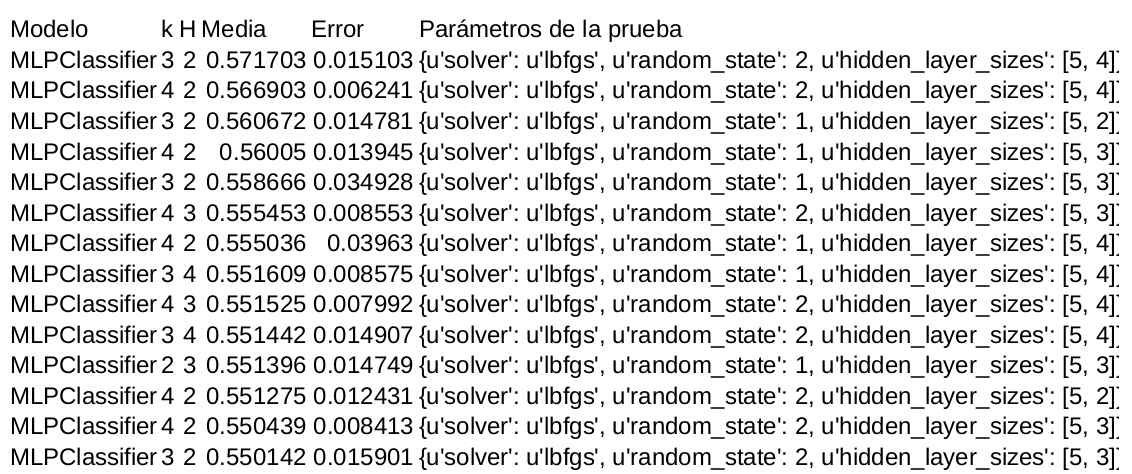
\includegraphics[width=14cm]{figures/resultado_mlp.png}
		\caption{Resultado redes neuronales \label{resultado_mlp}}
	\end{center}
\end{figure}

Una vez realizadas las pruebas, se observa que la media es muy baja,0.539901 en el mejor caso. Descartamos utilizar estos modelos de redes neuronales en nuestro proyecto.

Como futura vía de estudio se plantea volver a realizar este entrenamiento replanteando los parámetros y el ``mapeo'' de las clases.

Finalmente, hemos elegido el modelo SVR con las configuraciones siguientes:

\begin{itemize}
	\item k: 4
	\item distancia: 2
	\item kernel: ``rbf''
	\item C: 1000
	\item gamma: 0.001
\end{itemize}

\begin{figure}[htb]
	\begin{center}
		\includegraphics[width=16cm]{figures/resultado_elegido.png}
		\caption{Resultado elegido \label{resultado_elegido}}
	\end{center}
\end{figure}

Aunque no es el modelo con más media ni menos error, es de los más equilibrados. Esta configuración obtiene una media de acierto de 0.901516, distanciándose en 0.008493 de la media máxima conseguida. Su error es de 0.000330. Además se intuye que SVR debería ser el modelo que mejor se ajuste. Por lo que en un futuro estudio que busque mejorar esta predicción, sería un buen punto de partida.

\section{Calidad del código}
\label{makereference6.3}

Una vez acabado el código del proyecto, decidimos certificar su calidad mediante \href{https://www.codacy.com}{Codacy}.
Codacy es una herramienta que proporciona nuestro controlador de versiones GitHub. Sencillamente revisa todas y cada una de las líneas del código, para hacerlo más sencillo, escalable y seguro. Genera un informe con los errores y te dice qué grado de calidad tiene, siendo A el más alto. (\cite{ARP:Codacy:2017})

\begin{figure}[htb]
	\begin{center}
		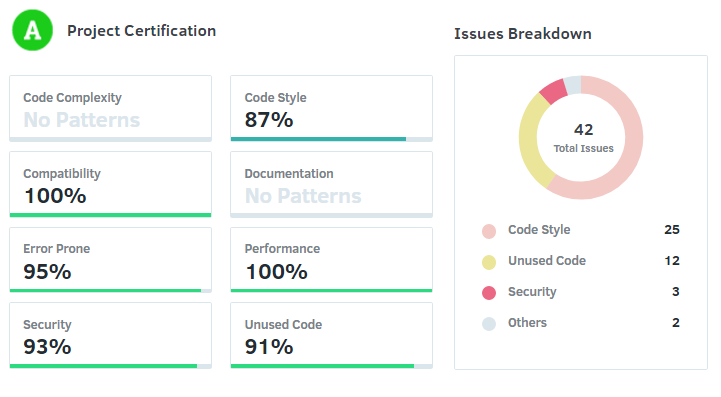
\includegraphics[height=3.5in]{figures/codacy.png}
		\caption{Informe de nuestro proyecto [Fuente: \href{https://www.codacy.com}{Codacy}] \label{codacy}}
	\end{center}
\end{figure}
\cleardoublepage

\chapter{Resultados}
\label{makereference7}

Los resultados de este apartado se basan en la exploración tipo Grid descrita en el apartado anterior. Los datos utilizados en esta exploración han sido los proporcionados por InfoRiego entre el 1 de enero de 2015 hasta el 31 de diciembre del 2015.

Para llevar a cabo el entrenamiento anterior, y poder obtener una métrica con la que evaluarlo, es necesario realizar una división del conjunto de datos en dos para cada prueba. Un conjunto para entrenar el modelo y otro para comprobar la precisión de este. Es importante que estos dos conjuntos sean complementarios ya que el modelo entrenado no debe conocer ningún dato del conjunto de test o el entrenamiento se vería alterado por conocer de antemano los datos a predecir.

El tamaño de cada conjunto es también un hecho relevante ya que con un conjunto de datos muy pequeño para el entrenamiento, la predicción sería dificilmente alcanzable con éxito y con un conjunto muy grande, habría pocos datos para probar que el modelo es fiable. Una división típica es dividir el conjunto de datos en 70/30, es decir, 70\% de los datos para entrenamiento y 30\% para comprobación. En este se ha utilizado una división 25/75 que es la utilizada por defecto por el grid search de SciKitLean.

Para poder analizar los resultados, la prueba anterior proporciona distintas métricas para medir la calidad del modelo. La implementación de GridSearch utilizada (librería de scikit-learn) pretende dar una misma interfaz para utilizar esta técnica con distintos algoritmos, por lo tanto, los resultados que se obtienen con ellos también tienen una misma forma de nombrar las métricas para todos.

Sin embargo, aunque en los ficheros de resultados aparezcan los mismos nombres para medir los resultados, el significado de estos es distinto dependiendo del modelo seleccionado. En los distintos apartados dedicados a cada uno de estos modelos se explicará el significado de sus métricas.

Junto con las métricas de calidad del modelo entrenado aparecen los parámetros necesarios para obtener dicho modelo. Tanto los parámetros específicos de cada modelo como el número de instantes anteriores utilizados (``k'') o la distancia a la predicción.

A la distancia a la predicción la llamaremos ``horizonte de predicción'' y especifica la diferencia entre la hora a la que se realiza la predicción y la hora a la que se quiere predecir entre el intervalo de medida (30 minutos para estos datos). Aunque se haya probado con varios horizontes, el que más nos interesa es ``2'', que indica una predicción a una hora.

Se han realizado tres conjuntos de pruebas, una por cada algoritmo predictivo estudiado. A continuación se analizan los resultados para cada uno de estos algoritmos.

\section{Regresión Lineal}
\label{makereference7.1}
Los parámetros suministrados a GridSearch para realizar el entrenamiento con este modelo son los siguientes:

\begin{itemize}
\item Inicio: 01-01-2015
\item Fin: 31-12-2015
\item k: 2, 3, 4, 5
\item Horizonte de predicción: 2, 3, 4, 5, 6, 7
\item fit\_intercept: true, false
\item copy\_X: true, false 
\end{itemize}

Grid serach estudiará los resultados para todas las combinaciones posibles.

De los resultados obtenidos para este algoritmo mostrados en la figura \ref{resultado_linear}, la columna ``mean'' nos indican el \(R^{2}\) obtenido. \(R^{2}\) es el coeficiente de correlación y, en regresión lineal, es el cuadrado del \textit{coeficiente de correlación de Pearson}. Se calcula dividiendo el cuadrado de la covarianza del conjunto de datos reales y los predichos entre el producto de los cuadrados de la desviación típica de cada conjunto. Expresa la calidad de la predicción del modelo entre 0 y 1.

\begin{figure}[htb]
	\begin{center}
		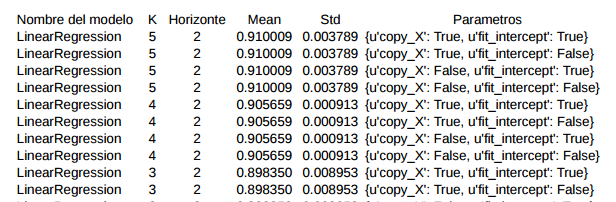
\includegraphics[width=14cm]{figures/resultado_linear.png}
		\caption{Resultado Regresión Lineal \label{resultado_linear}}
	\end{center}
\end{figure}

Los datos se muestran ordenados por la columna ``mean'' siendo así el primero de estos registros el que más coeficiente de correlación obtiene con un coeficiente de correlación de 0.910009.

Como se puede observar en la figura \ref{resultado_linear}, el modelo obtenido con mejor coeficiente de correlación tiene la siguiente configuración:

\begin{itemize}
\item Inicio: 01-01-2015
\item Fin: 31-12-2015
\item k: 5
\item Horizonte: 2
\item copy\_X: true
\item fit\_intercept: True
\end{itemize}

En el capítulo \ref{Appendix:Key1} (Anexo: Gráficas Regresión Lineal), se muestran distintas gráficas con la radiación de este modelo durante varios días del año, la predicción que obtenemos con el modelo obtenido con mayor coeficiente de correlación y el modelo conservador.

Este ``modelo conservador'' expresa una predicción de la radiación que toma como valor, la radiación que toma como predicción la radiación en el instante anterior.

El objetivo de este proyecto es superar, como mínimo este modelo conservador.

% TODO - Hablar sobre mean square error

\section{SVR}
\label{makereference7.2}

Para la exploración del modelo SVR usamos los siguientes parámetros:

\begin{itemize}
\item Inicio: 01-01-2015
\item Fin: 31-12-2015
\item k: 2, 3, 4, 5
\item Horizonte de predicción: 2, 3, 4, 5, 6, 7
\item C: 1, 10, 100, 1000
\item gamma: 0.001, 0.0001
\item kernel: linear, rbf 
\end{itemize}

En los resultados de la exploración mostrados en la figura \ref{resultado_svr}, la columna ``mean'' utiliza la misma métrica que la vista en el apartado anterior. Esto es porque ambas son regresiones y esta es muy utilizada en ese caso.

\begin{figure}[htb]
	\begin{center}
		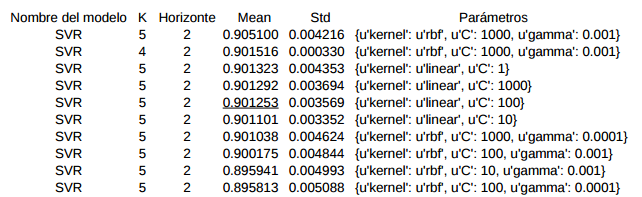
\includegraphics[width=14cm]{figures/resultado_svr.png}
		\caption{Resultado Regresión Lineal \label{resultado_svr}}
	\end{center}
\end{figure}

La figura \ref{resultado_svr} muestra el modelo obtenido con mejor coeficiente de correlación (0.905100) y su configuración:

\begin{itemize}
\item Inicio: 01-01-2015
\item Fin: 31-12-2015
\item k: 5
\item Horizonte de predicción: 2
\item C: 1000
\item gamma: 0.0001
\item kernel: rbf 
\end{itemize}

En el capítulo \ref{Appendix:Key2} (Anexo: Gráficas SVR) podemos observar varias gráficas para distintos días del año con la predicción obtenida con este modelo frente a la radiación real y al modelo conservador.

% TODO hay que interpretar la gráfica. ¿falla mucho el modelo? ¿falla más al amanecer/atardecer?¿falla más en verano? ¿se ve facilmente cuándo falla más? 
%creo que falla más cuando más variaciones repentinas hay (cuando hay más picos hacia abajo)

% Explicar que "MSE" es mean square error que significa el error medio al cuadrado. Es la media de las restas entre la prediccion y lo real al cuadrado. Para poder ver cuándo falla más y cuándo menos, se puede ver cuándo tiene menor MSE.

% Hacer esto para los tres modelos

\section{Redes Neuronales}
\label{makereference7.3}

En la figura \ref{json_mlp} se puede observar los parámetros a explorar que usa GridSearch para determinar qué configuración del modelo de redes neuronales es mejor para nuestro proyecto:

\begin{itemize}
\item Inicio: 01-01-2015
\item Fin: 31-12-2015
\item k: 2, 3, 4, 5
\item Horizonte de predicción: 2, 3, 4, 5, 6, 7
\item solver: lbfgs, sgd
\item hidden\_layers: (5, 2), (5, 3), (5, 4)
\item ramdon\_state: 1, 2
\end{itemize}

En este caso, la métrica utilizada para determinar la calidad del modelo ha sido ``accuracy'' (en español, exactitud). Es una métrica muy utilizada en clasificadores que indica el porcentaje de predicciones clasificadas correctamente.

\begin{figure}[htb]
	\begin{center}
		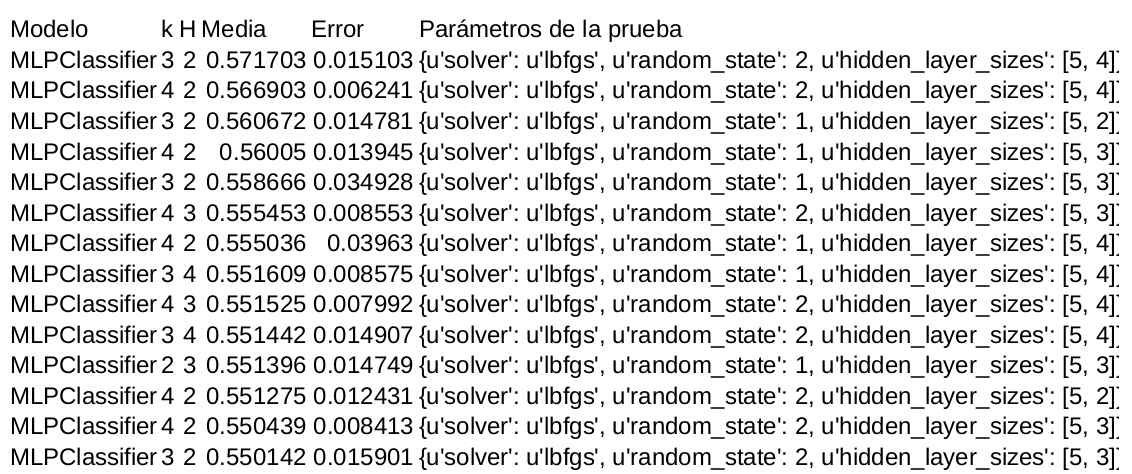
\includegraphics[width=17cm]{figures/resultado_mlp.png}
		\caption{Resultado redes neuronales \label{resultado_mlp}}
	\end{center}
\end{figure}

En la figura \ref{resultado_mlp} podemos ver los resultados del grid search para Redes Neuronales. La configuración del modelo con mayor ``accuracy'' obtenido es la siguiente:

\begin{itemize}
\item Inicio: 01-01-2015
\item Fin: 31-12-2015
\item k: 3
\item Horizonte de predicción: 2
\item solver: lbfgs
\item hidden\_layers: (5, 4)
\item ramdon\_state: 2
\end{itemize}

En el capítulo \ref{Appendix:Key3} tenemos distintas gráficas con la predicción realizada por este modelo, la radiación real y la predicción del modelo conservador para distintos días del año 2016.

% TODO hablar de mean square error y gráficas

\section{Calidad del código}
\label{makereference7.4}

Una vez acabado el código del proyecto, decidimos certificar su calidad mediante \href{https://www.codacy.com}{Codacy}.
Codacy es una herramienta que proporciona nuestro controlador de versiones GitHub. Sencillamente revisa todas y cada una de las líneas del código, para hacerlo más sencillo, escalable y seguro. Genera un informe con los errores y te dice qué grado de calidad tiene, siendo A el más alto. (\cite{ARP:Codacy:2017})

\begin{figure}[htb]
	\begin{center}
		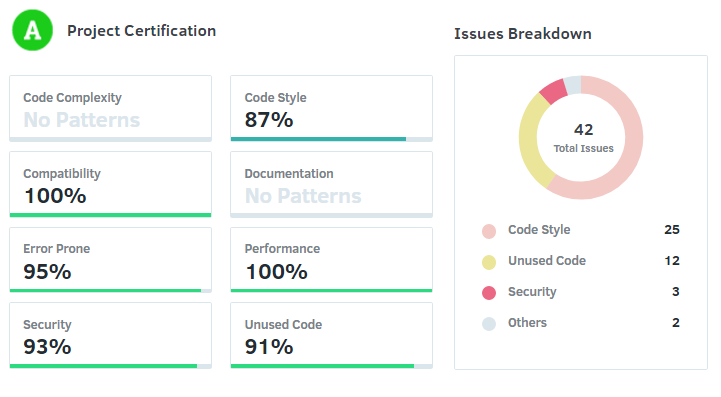
\includegraphics[height=3.5in]{figures/codacy.png}
		\caption{Informe de nuestro proyecto [Fuente: \href{https://www.codacy.com}{Codacy}] \label{codacy}}
	\end{center}
\end{figure}
\cleardoublepage

\chapter{Conclusiones}
\label{makereference8}

\section{Estado del proyecto}

Los hitos que hemos conseguido desarrollar con éxito son:
\begin{itemize}
\item Montar un sistema de recogida de datos. Un nodo muy sencillo de replicar y que fácilmente podría trabajar en una red de estos. Gracias al protocolo MQTT que permite muchos ``publicadores'' y a que a la hora del entrenamiento se ha tenido en cuenta el identificador del nodo con el que se ha trabajado, se podría añadir al estudio los datos recogidos por múltiples nodos a lo largo de una extensión de terreno.

\item Sistema de entrenamiento de datos. El software desarrollado para la obtención y tratamiento de los datos para el entrenamiento permite obtener conjuntos de datos de forma parametrizada. De esta forma, en una posible continuación del proyecto, sería muy sencillo generar sus propios conjuntos de datos para el entrenamiento. Además se han explorado ciertos modelos predictivos que, aún sin mucho éxito, no haría falta volver a estudiar con nuestros parámetros.

\item Sistema de predicción. Aunque no se haya conseguido un modelo de predicción óptimo, sí se ha desarrollado el sistema que recibe los datos recogidos y utiliza el modelo elegido para realizar una predicción. Además, debido a la modularidad de nuestro sistema, es muy sencillo implementar nuevos modelos de predicción.
\end{itemize}

Cada uno de los componentes del sistema se ha desarrollado pensando en una posible futura sustitución o mejora. Asi, cada componente es autónomo y fácilmente reemplazable por otro que respete la interfaz de comunicación. Esto permite que las posibles carencias puedan ser solventadas sin la necesidad de alterar el resto de componentes.

Este proyecto deja un margen de mejora sobre los requisitos inciales:
\begin{itemize}
\item Modelo predictivo. No se ha logrado obtener una predicción suficiente como para poder llevar este sistema a un entorno real. Una de las posibles mejoras sería estudiar otros modelos y parámetros.

\item Sistema de visualización. Debido a la falta de tiempo para tomar muestras del nodo, no se ha podido pulir este componente. La información que muestra no aparece de una forma clara. Sin embargo, sí recibe y almacena los datos necesarios y en un futuro sólo sería necesario corregir el fragmento de código que transforma los datos crudos en gráficas representativas.
\end{itemize}

\section{Posibles ampliaciones}
Desde un primer momento, se tenía como una posible ampliación formar una red de nodos para la recogida de muestras. Se ha empezado por desarrollar uno para no ampliar la complejidad del proyecto.

Se intuye que dentro del modelo predictivo, podría ser interesante disponer de muestras desde distintos puntos de un territorio. Quizá esto podría permitir inferir al modelo predictivo cambios en las condiciones meteorológicas en un nodo a partir de las recogidas por otro.

Por último, otra posible ampliación, sería estudiar el modelo de predicción \href{https://www.analyticsvidhya.com/blog/2016/02/time-series-forecasting-codes-python/}{ARIMA}. Que hace uso de regresión lineal teniendo en cuenta valores pasados.
\cleardoublepage

\chapter{Conclusions}
\label{makereference9}

\section{Project status}

The milestones we have successfully developed are:
\begin{itemize}
\item Set up a data collection system. A very simple node to replicate and it could easily work on a network of these. Thanks to the MQTT protocol that allows many publishers since at the time of the training, the identifier of the node with which it was worked was taken into account, the data collected by multiple nodes could be added to the study. An extension of land.

\item Data training system. The software developed for obtaining and processing data for training allows to obtain data sets in a parameterized way. In this way, in a possible continuation of the project, it would be very easy to generate their own data sets for training. In addition, we have explored certain predictive models that, even without much success, would not need to re-study with our parameters.

\item Prediction system. Although an optimal prediction model has not been achieved, the system that receives the collected data has been developed and uses the model chosen to make a prediction. In addition, due to the modularity of our system, it is very easy to implement new prediction models.
\end{itemize}

Each of the components of the system has been developed with a possible future replacement or improvement. Thus, each component is autonomous and easily replaceable by another that respects the communication interface. This allows that the possible deficiencies can be solved without the necessity to alter the rest of components.

This project leaves a margin of improvement over the initial requirements:

\begin{itemize}
\item Predictive model. It has not been possible to obtain a prediction sufficient to be able to take this system to a real environment. One of the possible improvements would be to study other models and parameters.

\item Display system. Due to the lack of time to sample the node, this component could not be polished. The information shown does not appear clearly. However, it does receive and store the necessary data and in the future it would only be necessary to correct the piece of code that transforms raw data into representative charts.
\end{itemize}

\section{Possible extensions}
From the outset, it was possible to form a network of nodes for the collection of samples. It has begun to develop one so as not to expand the complexity of the project.

It is intuited that within the predictive model, it could be interesting to have samples from different points of a territory. Perhaps this could allow to infer to the predictive model changes in the meteorological conditions in a node from those collected by another.

Finally, another possible extension would be to study the prediction model \href{https://www.analyticsvidhya.com/blog/2016/02/time-series-forecasting-codes-python/}{ARIMA}. It makes use of linear regression taking into account past values.
\cleardoublepage

\chapter{Conclusions}
\label{makereference10}

\section{Project status}

The milestones we have successfully developed are:
\begin{itemize}
\item Set up a data collection system. A very simple node to replicate and it could easily work on a network of these. Thanks to the MQTT protocol that allows many publishers since at the time of the training, the identifier of the node with which it was worked was taken into account, the data collected by multiple nodes could be added to the study. An extension of land.

\item Data training system. The software developed for obtaining and processing data for training allows to obtain data sets in a parameterized way. In this way, in a possible continuation of the project, it would be very easy to generate their own data sets for training. In addition, we have explored certain predictive models that, even without much success, would not need to re-study with our parameters.

\item Prediction system. Although an optimal prediction model has not been achieved, the system that receives the collected data has been developed and uses the model chosen to make a prediction. In addition, due to the modularity of our system, it is very easy to implement new prediction models.
\end{itemize}

Each of the components of the system has been developed with a possible future replacement or improvement. Thus, each component is autonomous and easily replaceable by another that respects the communication interface. This allows that the possible deficiencies can be solved without the necessity to alter the rest of components.

This project leaves a margin of improvement over the initial requirements:

\begin{itemize}
\item Predictive model. It has not been possible to obtain a prediction sufficient to be able to take this system to a real environment. One of the possible improvements would be to study other models and parameters.

\item Display system. Due to the lack of time to sample the node, this component could not be polished. The information shown does not appear clearly. However, it does receive and store the necessary data and in the future it would only be necessary to correct the piece of code that transforms raw data into representative charts.
\end{itemize}

\section{Possible extensions}
From the outset, it was possible to form a network of nodes for the collection of samples. It has begun to develop one so as not to expand the complexity of the project.

It is intuited that within the predictive model, it could be interesting to have samples from different points of a territory. Perhaps this could allow to infer to the predictive model changes in the meteorological conditions in a node from those collected by another.

Finally, another possible extension would be to study the prediction model \href{https://www.analyticsvidhya.com/blog/2016/02/time-series-forecasting-codes-python/}{ARIMA}. It makes use of linear regression taking into account past values.
\cleardoublepage

\chapter{Trabajo del Alumno}
\label{makereference11}

\section{Pablo Aragón Moreno}
\subsection{Investigación}
\subsection{Desarrollo}
\subsection{Documentación}


\section{María Castañeda López}
\subsection{Investigación}
\subsection{Desarrollo}
\subsection{Documentación}


\section{Abel Coronado López}
\subsection{Investigación}

Durante la fase inicial del proyecto, Abel Coronado López se encargó de la investigación de las distintas tecnologías para desarrollar ``Machine Learning'' que se encontraban actualmente en el ``mercado'' y seleccionar cuál era la que mejor le venía al proyecto, y cuáles eran los motivos por los que había escogido la tecnología.

En un principio, la tecnología a utilizar sería MATLAB, pero, después de la investigación previa, se descubrió que Python también tiene una gran potencia en este sector. Python cuenta con un gran abanico de librerías para trabajar con grandes cantidades de datos, análisis científico, inteligencia artificial... Cuenta también con distribuciones que ya incluyen gran cantidad de estas librerías para poder hacer uso de ellas sin necesidad de instalarlas una a una como ``Anaconda''. Además, junto con la facilidad de programar en este lenguaje y la experiencia previa de los componentes del grupo con él, hizo que esta fuera la elección final.

Tras tener elegida la tecnología con la que desarrollar el proyecto, Abel Coronado López, investigó distintos algoritmos matemáticos para el ``Machine Learning'' y cómo poder implementarlos.

Hizo uso de cursos online, como por ejemplo \href{https://www.udacity.com}{Udacity}, y se valió de tutoriales básicos de ``Machine Learning'' en \href{https://www.youtube.com}{YouTube} para coger una idea básica de este nuevo paradigma emergente.

Con una idea más clara de los objetivos del proyecto y de cómo implementarlos, el alumno estudió pequeños problemas resueltos relacionados con la IA propuestos en Intenet:

\begin{itemize}
\item Desastre del Titanic
\item Investigación de la diabetes
\item Predicción del divorcio
\end{itemize}

Cuando la fase de estudio de los algoritmos concluyó, el alumno, junto al resto de componentes del equipo, generó una lista de posibles algoritmos para utilizar en el proyecto: 

\begin{itemize}
\item Regresión Lineal
\item SVM
\item Clasificador
\end{itemize}

Esta lista iría cambiando según avanzara el proyecto debido a diversos factores:

\begin{itemize}
\item Poca documentación
\item Problemas de implementación
\item Malos resultados
\end{itemize}

En esta fase de investigación, se descubrió un método de estudio para automatizar las pruebas y hacer más viable la experimentación de modelos y parámetros usados en el ``Machine Learning'': Grid Search \ref{makereference5.3}.

\subsection{Desarrollo}
Con la fase de investigación finalizada, Abel Coronado López, junto con el resto de compañeros, empezaron con el desarrollo e implementación de estos algoritmos en el proyecto.

Gracias a Grid Seach este trabajo fue mucho más viable y cómodo.

Se desarrolló una plantilla que usa Grid Search para abstraer los modelos y parámetros a explorar. De esta manera, la fase de entrenamiento sería configurable mediante archivos ``JSON''. El alumno desarrolló dichos ficheros explicados previamente. Ver figura \ref{json}.

Una vez finalizada la fase de entrenamiento con distintos modelos y configuraciones, el equipo eligió el algoritmo que mejor precisión de predicción tiene para nuestro contexto.

\subsection{Documentación}
Durante todos los procesos anteriormente descritos, el alumno Abel Coronado López documentó todo lo relacionado con las tecnologías investigadas y utilizadas por el sistema en una carpeta compartida por el equipo de desarrollo del proyecto, y en Github. Esta documentación consistía en comentar todo lo que se iba desarrollando e investigando, de forma que los demás compañeros, si querían introducirse en esa parte del sistema, únicamente tendrían que leer dónde y cómo se hizo.

En la fase final del proyecto, el alumno ha documentado todo el sistema relacionado con la predicción para que este fuese introducido en la memoria del proyecto, también a aportado en otras secciones como la introducción, el nodo, etc...

%\bibliographystyle{styles/plain}
\bibliographystyle{styles/plain}

%\bibdata{references}
\bibliography{references}
%\addcontentsline{toc}{chapter}{Bibliography}

%\appendix
%% +--------------------------------------------------------------------+
% | Appendix A Page (Optional)                                         |
% +--------------------------------------------------------------------+

\cleardoublepage

\chapter{Anexo: Gráficas Regresión Lineal}
\label{Appendix:Key1}


% +--------------------------------------------------------------------+
% | Enter text for your Appendix page in the space below this box.     |
% |                                                                    |
% +--------------------------------------------------------------------+

\begin{figure}[htb]
\minipage{0.5\textwidth}
		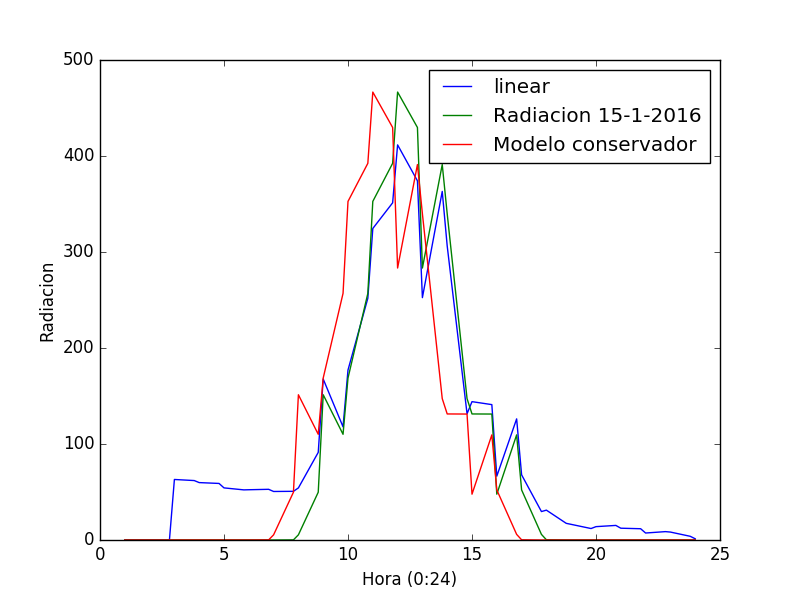
\includegraphics[width=\linewidth]{figures/linear_2016011520160115.png}
		\caption{Resultado 15-01-2016 \label{resultado_linear_1}}
\endminipage\hfill
\minipage{0.5\textwidth}
		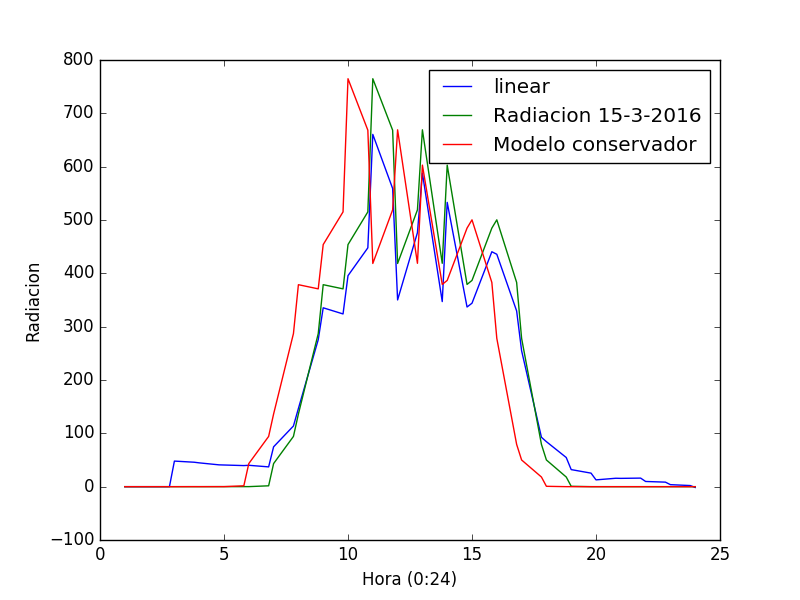
\includegraphics[width=\linewidth]{figures/linear_2016031520160315.png}
		\caption{Resultado 15-03-2016 \label{resultado_linear_2}}
\endminipage\hfill
\end{figure}

\begin{figure}[htb]
\minipage{0.5\textwidth}
		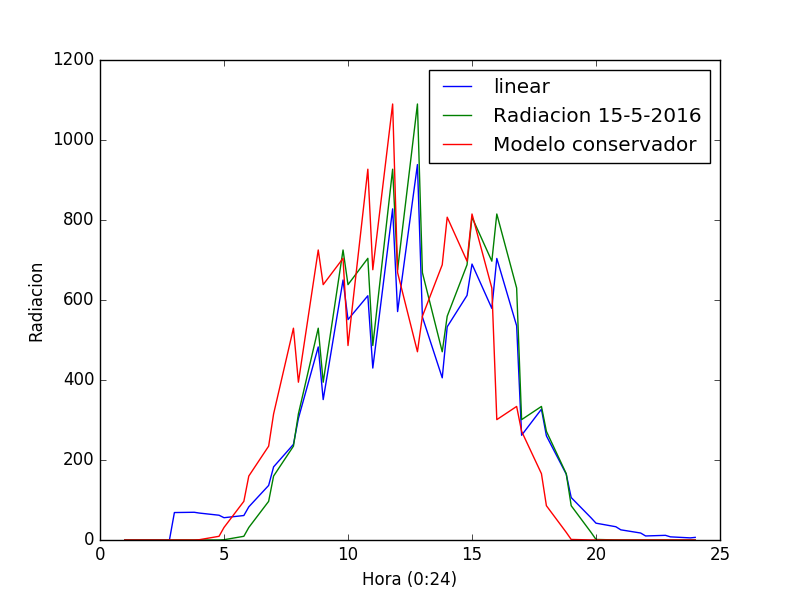
\includegraphics[width=\linewidth]{figures/linear_2016051520160515.png}
		\caption{Resultado 15-05-2016 \label{resultado_linear_3}}
\endminipage\hfill
\minipage{0.5\textwidth}
		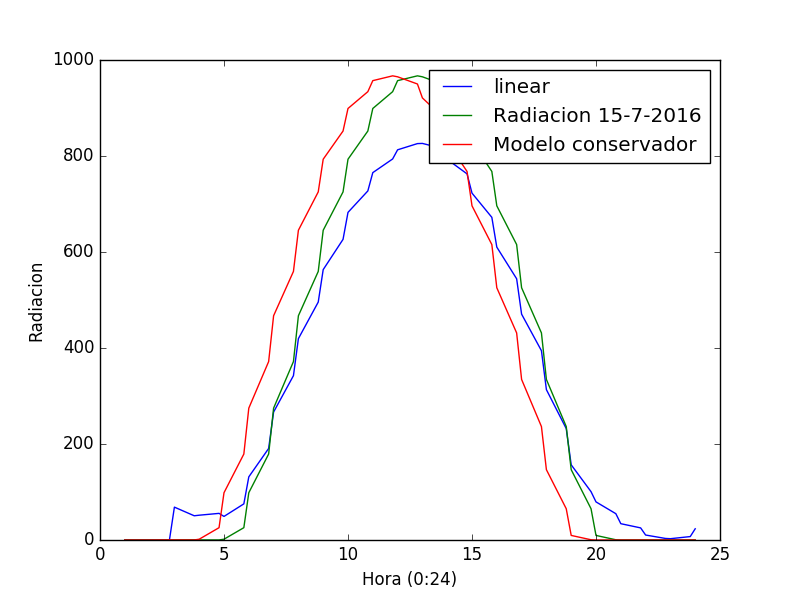
\includegraphics[width=\linewidth]{figures/linear_2016071520160715.png}
		\caption{Resultado 15-07-2016 \label{resultado_linear_4}}
\endminipage\hfill
\end{figure}

\begin{figure}[htb]
\minipage{0.5\textwidth}
		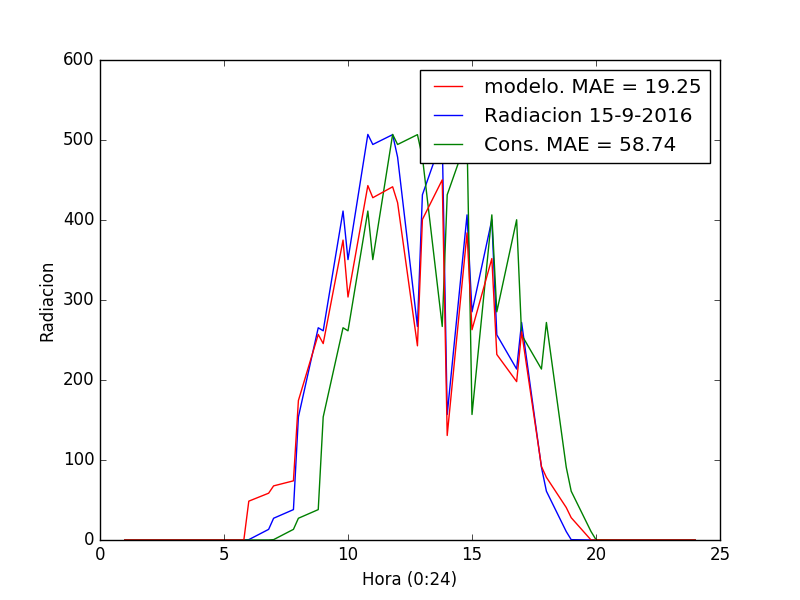
\includegraphics[width=\linewidth]{figures/linear_2016091520160915.png}
		\caption{Resultado 15-09-2016 \label{resultado_linear_5}}
\endminipage\hfill
\minipage{0.5\textwidth}
		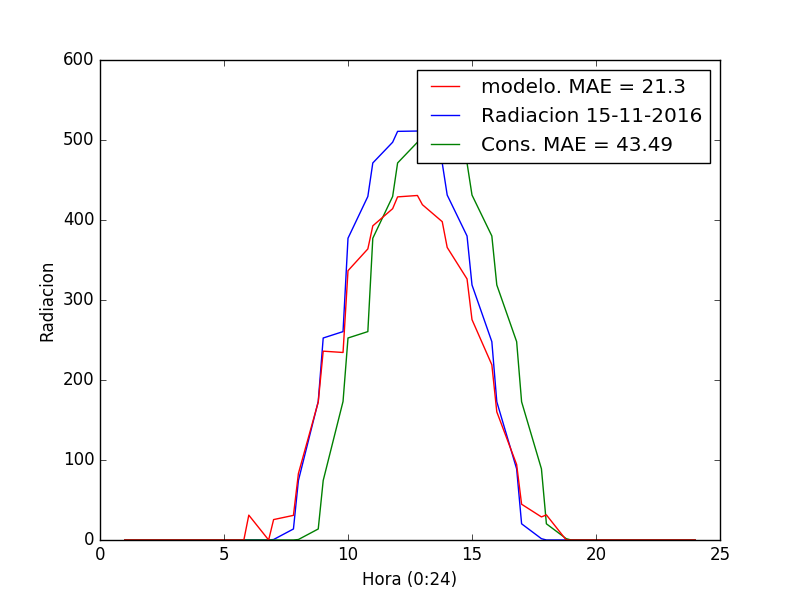
\includegraphics[width=\linewidth]{figures/linear_2016111520161115.png}
		\caption{Resultado 15-11-2016 \label{resultado_linear_6}}
\endminipage\hfill
\end{figure}

\chapter{Anexo: Gráficas SVR}
\label{Appendix:Key2}

\begin{figure}[htb]
\minipage{0.5\textwidth}
		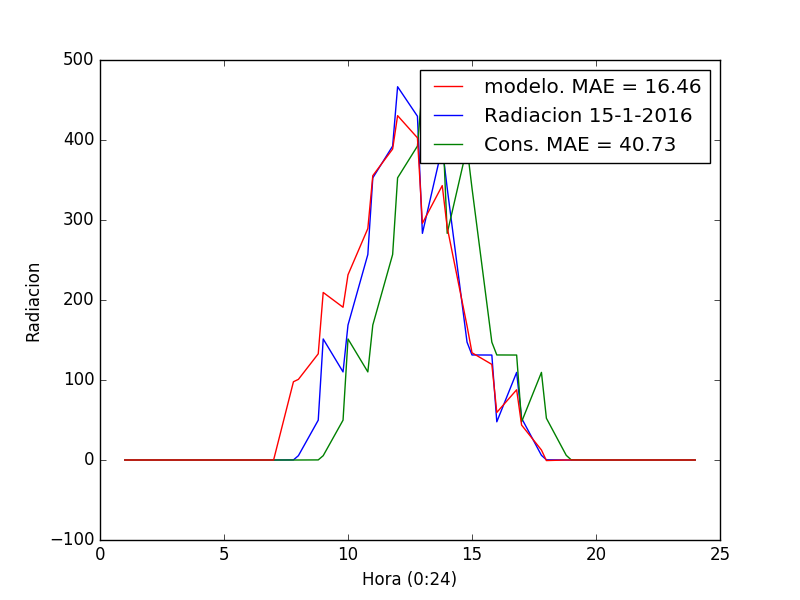
\includegraphics[width=\linewidth]{figures/svr_2016011520160115.png}
		\caption{Resultado 15-01-2016 \label{resultado_svr_1}}
\endminipage\hfill
\minipage{0.5\textwidth}
		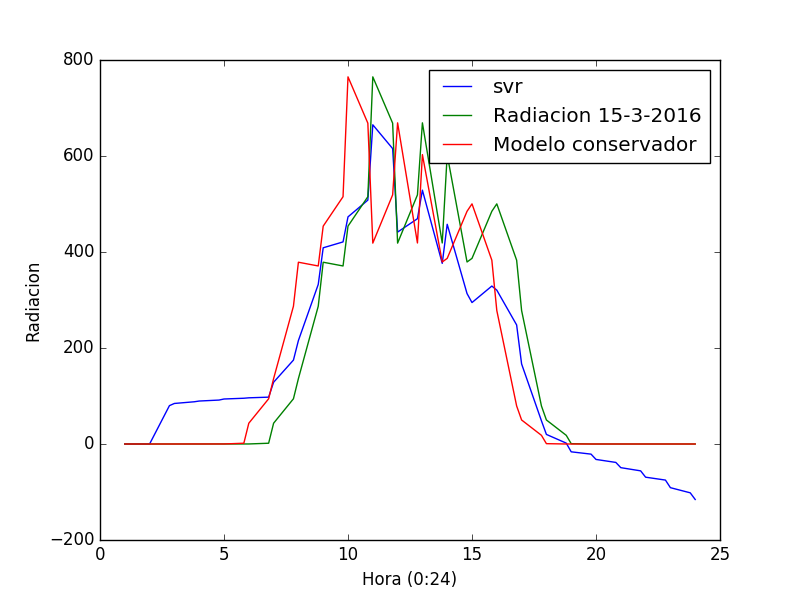
\includegraphics[width=\linewidth]{figures/svr_2016031520160315.png}
		\caption{Resultado 15-03-2016 \label{resultado_svr_2}}
\endminipage\hfill
\end{figure}

\begin{figure}[htb]
\minipage{0.5\textwidth}%
		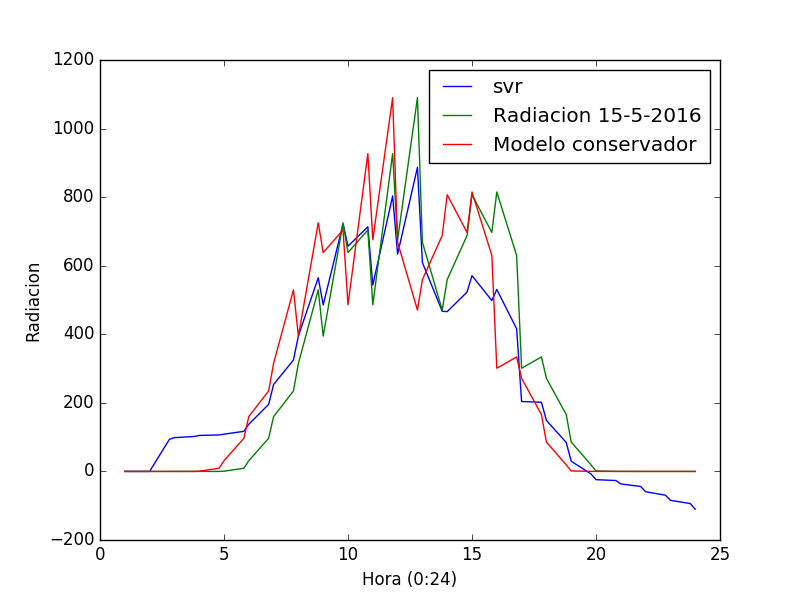
\includegraphics[width=\linewidth]{figures/svr_2016051520160515.png}
		\caption{Resultado 15-05-2016 \label{resultado_svr_3}}
\endminipage\hfill
\minipage{0.5\textwidth}%
		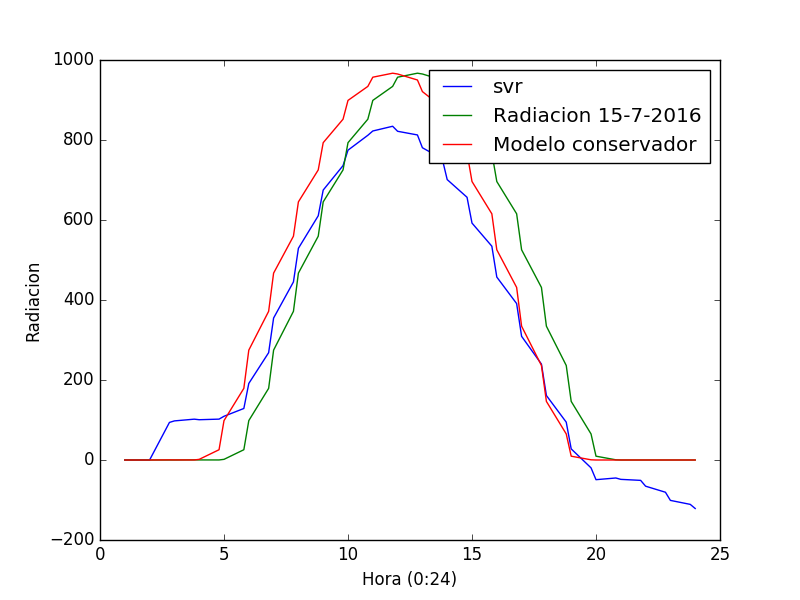
\includegraphics[width=\linewidth]{figures/svr_2016071520160715.png}
		\caption{Resultado 15-07-2016 \label{resultado_svr_4}}
\endminipage\hfill
\end{figure}
\begin{figure}[htb]
\minipage{0.5\textwidth}%
		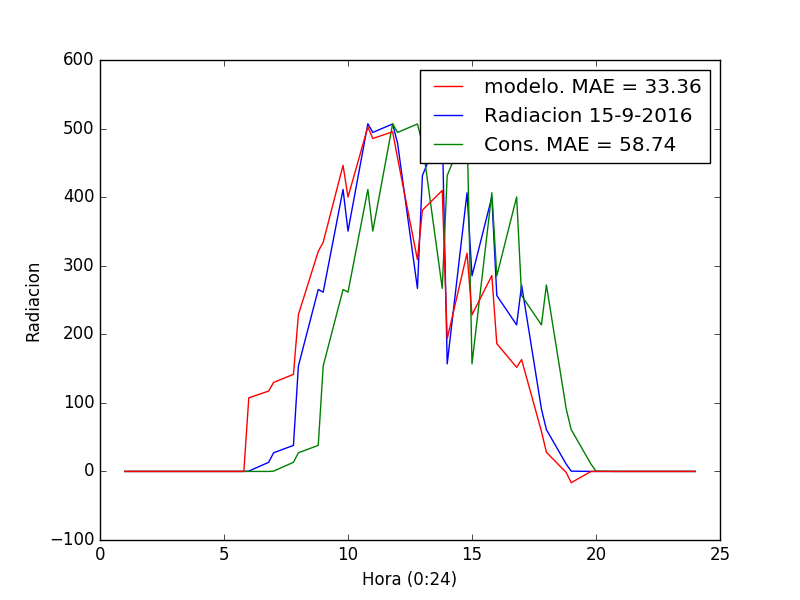
\includegraphics[width=\linewidth]{figures/svr_2016091520160915.png}
		\caption{Resultado 15-09-2016 \label{resultado_svr_5}}
\endminipage\hfill
\minipage{0.5\textwidth}%
		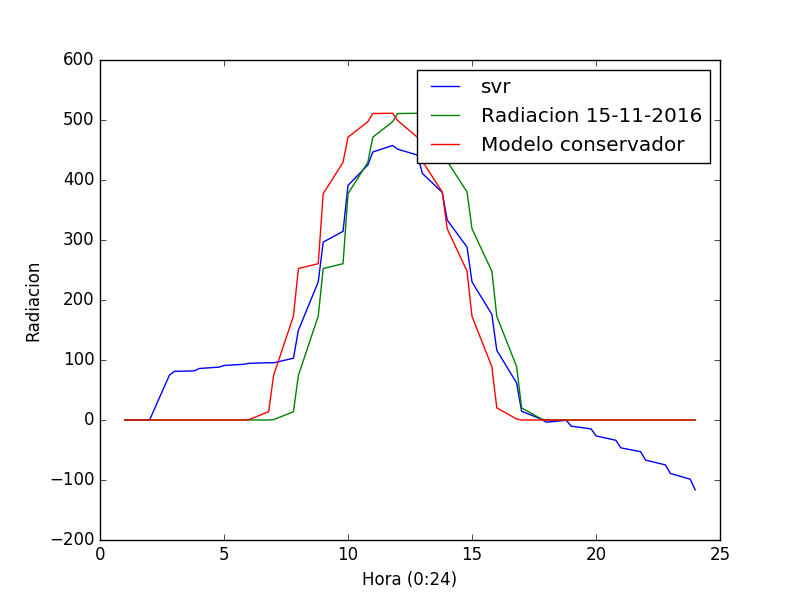
\includegraphics[width=\linewidth]{figures/svr_2016111520161115.png}
		\caption{Resultado 15-11-2016 \label{resultado_svr_6}}
\endminipage
\end{figure}

\chapter{Anexo: Gráficas Redes Neuronales}
\label{Appendix:Key3}

\begin{figure}[htb]
\minipage{0.5\textwidth}
		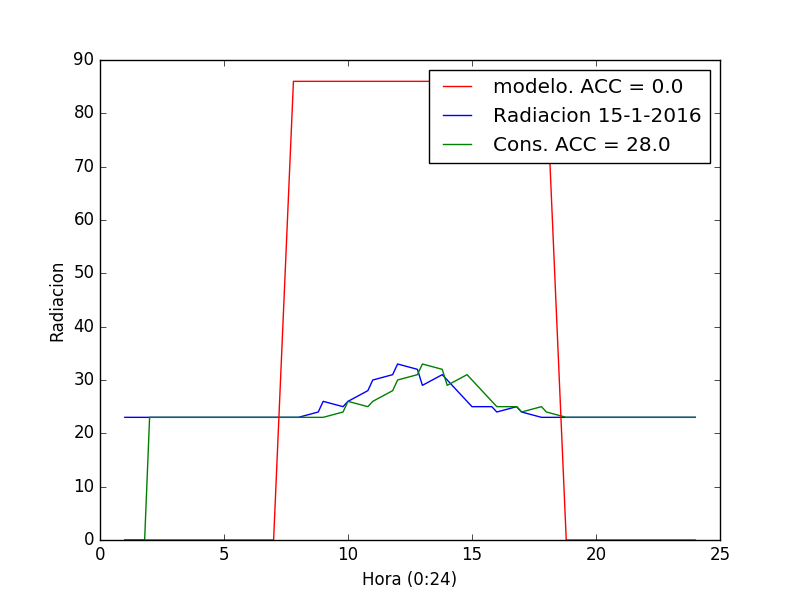
\includegraphics[width=\linewidth]{figures/mlp_2016011520160115.png}
		\caption{Resultado 15-01-2016 \label{resultado_mlp_1}}
\endminipage\hfill
\minipage{0.5\textwidth}
		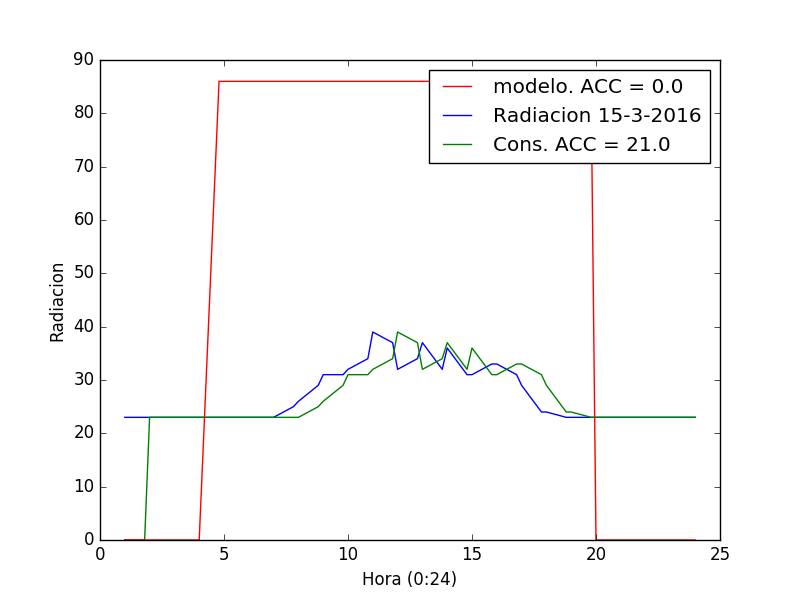
\includegraphics[width=\linewidth]{figures/mlp_2016031520160315.png}
		\caption{Resultado 15-03-2016 \label{resultado_mlp_2}}
\endminipage\hfill
\end{figure}

\begin{figure}[htb]
\minipage{0.5\textwidth}
		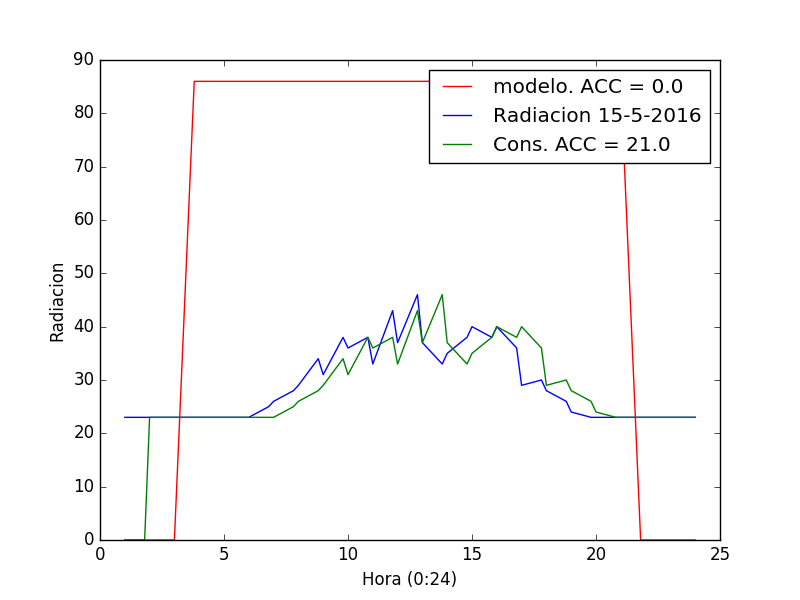
\includegraphics[width=\linewidth]{figures/mlp_2016051520160515.png}
		\caption{Resultado 15-05-2016 \label{resultado_mlp_3}}
\endminipage\hfill
\minipage{0.5\textwidth}
		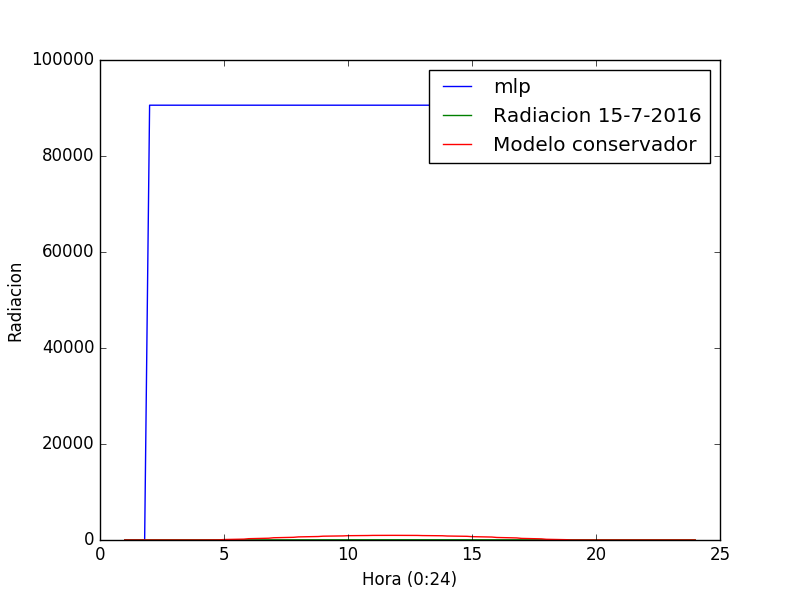
\includegraphics[width=\linewidth]{figures/mlp_2016071520160715.png}
		\caption{Resultado 15-07-2016 \label{resultado_mlp_4}}
\endminipage\hfill
\end{figure}

\begin{figure}[htb]
\minipage{0.5\textwidth}
		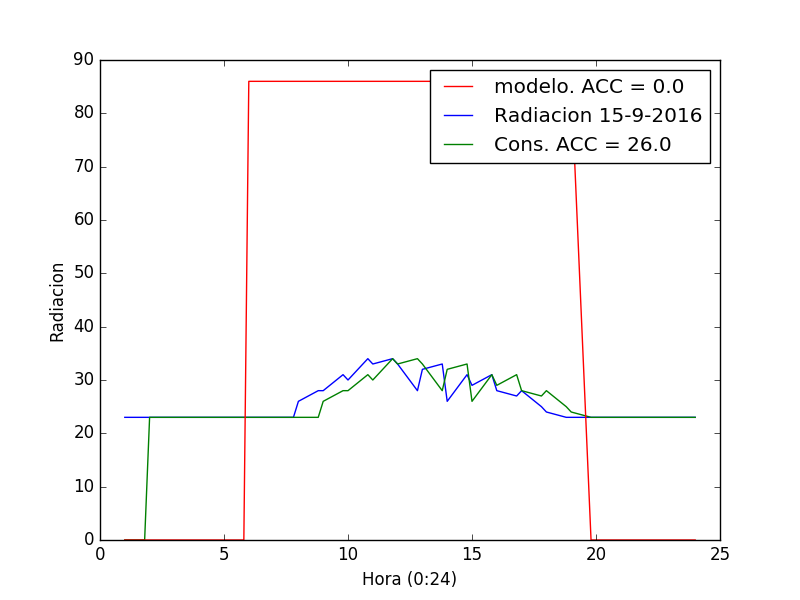
\includegraphics[width=\linewidth]{figures/mlp_2016091520160915.png}
		\caption{Resultado 15-09-2016 \label{resultado_mlp_5}}
\endminipage\hfill
\minipage{0.5\textwidth}
		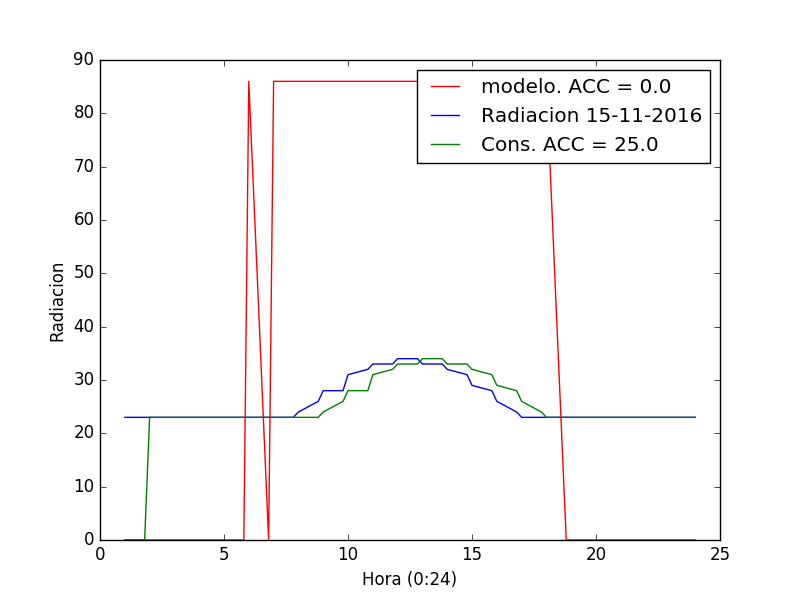
\includegraphics[width=\linewidth]{figures/mlp_2016111520161115.png}
		\caption{Resultado 15-11-2016 \label{resultado_mlp_6}}
\endminipage
\end{figure}

%% +--------------------------------------------------------------------+
% | Appendix B Page (Optional)                                         |
% +--------------------------------------------------------------------+

\cleardoublepage

\chapter{Anexo: Calidad del código}
\label{Appendix:Key2}

Una vez acabado el código del proyecto, decidimos certificar su calidad mediante \href{https://www.codacy.com}{Codacy}.
Codacy es una herramienta que proporciona nuestro controlador de versiones GitHub. Sencillamente revisa todas y cada una de las líneas del código, para hacerlo más sencillo, escalable y seguro. Genera un informe con los errores y te dice qué grado de calidad tiene, siendo A el más alto. (\cite{ARP:Codacy:2017})

\begin{figure}[htb]
	\begin{center}
		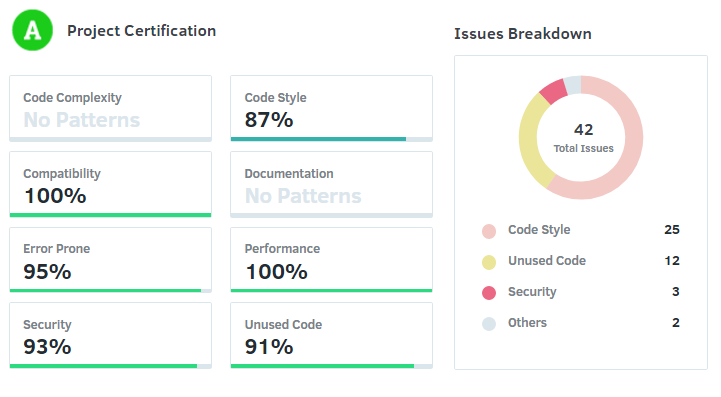
\includegraphics[height=3.5in]{figures/codacy.png}
		\caption{Informe de nuestro proyecto [Fuente: \href{https://www.codacy.com}{Codacy}] \label{codacy}}
	\end{center}
\end{figure}


\end{document}
